\subsection{Inverse limits of measures}

Let X, Y be two compact spaces, \(p : X \to Y\) a continuous mapping; then \(f \mapsto f \circ p\) is a continuous linear mapping of \(\mathcal{C}(Y; \mathbf{C})\) into \(\mathcal{C}(X; \mathbf{C})\) , since \(\|f \circ p\| \leqslant \|f\|\) for every function \(f \in \mathcal{C}(Y; \mathbf{C})\) ; we denote this mapping by \(p'\) . Its transpose \(^{t}p' : M(X; C) \to M(Y; C)\) is therefore such that, for every measure \(\mu\) on X, \(^{t}p'(\mu)\) is the measure on Y such that

\[
\langle^ {t} p ^ {\prime} (\mu), f \rangle = \langle \mu , f \circ p \rangle
\]

for every function \(f \in \mathcal{C}(\mathrm{Y};\mathbf{C})\) . Note that for every \(x \in \mathrm{X}\) , \(^t p'(\varepsilon_x) = \varepsilon_{p(x)}\) ; for this reason, we shall denote by \(p_*(\mu)\) the measure \(^t p'(\mu)\) , which thus extends \(p\) when \(\mathrm{X}\) (resp. \(\mathrm{Y}\) ) is canonically embedded in \(\mathcal{M}(\mathrm{X};\mathbf{C})\) (resp. \(\mathcal{M}(\mathrm{Y};\mathbf{C})\) ) (§1, No.~9, Prop. 13); for every measure \(\mu\) on \(\mathrm{X}\) , \(p_*(\mu)\) is a special case of the general concept of image of a measure, which we shall study in Ch. V, §6. Since, as we saw above, \(\| p' \| \leqslant 1\) , we have also \(\| ^t p' \| \leqslant 1\) and so

\[
\| p _ {*} (\mu) \| \leqslant \| \mu \|\tag{15}
\]

for every measure \(\mu \in \mathcal{M}(\mathrm{X};\mathbf{C})\)

Let us now consider a directed pre-ordered set I, and an inverse system (or `projective system') \((\mathrm{X}_{\alpha}, p_{\alpha\beta})\) of compact spaces \(X_{\alpha}\) (GT, I, §4, No.~4) having I as set of indices; the inverse limit space \(X = \varprojlim X_{\alpha}\) is known to be compact (GT, I, §9, No.~6, Prop. 8); we shall denote by \(p_{\alpha}\) the canonical mapping of X into \(X_{\alpha}\) .

It is clear that \((\mathcal{M}(\mathrm{X}_{\alpha};\mathbf{C}),(p_{\alpha\beta})_{*})\) is an inverse system of vector spaces, and that \(((p_{\alpha})_{*})\) is an inverse system of linear mappings, which justifies the following definition:

DEFINITION 2. --- A family \((\mu_{\alpha})_{\alpha \in I}\) , where, for every \(\alpha \in I\) , \(\mu_{\alpha}\) is a measure on \(X_{\alpha}\) , is said to be an inverse system of measures if, whenever \(\alpha \leqslant \beta\) , \(\mu_{\alpha} = (p_{\alpha \beta})_{*}(\mu_{\beta})\) . A measure \(\mu\) on \(X = \varprojlim X_{\alpha}\) is said to be an inverse limit of the inverse system \((\mu_{\alpha})\) if \(\mu_{\alpha} = (p_{\alpha})_{*}(\mu)\) for every \(\alpha \in I\) .

PROPOSITION 8. --- (i) If an inverse system \((\mu_{\alpha})\) of measures on the \(X_{\alpha}\) has an inverse limit, then that limit is unique.

\begin{enumerate}
\def\labelenumi{(\roman{enumi})}
\setcounter{enumi}{1}
\item
  If an inverse system \((\mu_{\alpha})\) has an inverse limit, then the family of norms \((\| \mu_{\alpha}\|)\) is bounded.
\item
  If the \(p_{\alpha\beta}\) are surjective and the family ( \(\|\mu_{\alpha}\|\) ) is bounded, then the inverse system of measures ( \(\mu_{\alpha}\) ) has an inverse limit.
\item
  If the \(p_{\alpha \beta}\) are surjective, then every inverse system \((\mu_{\alpha})\) of positive measures has an inverse limit \(\mu\) , which is a positive measure on \(X\) , and \(\| \mu \| = \| \mu_{\alpha} \|\) for all \(\alpha\) .
\end{enumerate}

\begin{enumerate}
\def\labelenumi{(\roman{enumi})}
\tightlist
\item
  We first prove the following lemma:
\end{enumerate}

Lemma 3. --- Let F be the set of functions \(f \in \mathcal{C}(\mathrm{X};\mathbf{C})\) having the following property: there exist an \(\alpha \in \mathrm{I}\) and a function \(f_{\alpha} \in \mathcal{C}(\mathrm{X}_{\alpha};\mathbf{C})\) such that \(f = f_{\alpha} \circ p_{\alpha}\) . Then F is a dense linear subspace of \(\mathcal{C}(\mathrm{X};\mathbf{C})\) .

We note first of all that if \(g = g_{\beta} \circ p_{\beta}\) and \(h = h_{\gamma} \circ p_{\gamma}\) , where \(g_{\beta} \in \mathcal{C}(\mathrm{X}_{\beta}; \mathbf{C})\) and \(h_{\gamma} \in \mathcal{C}(\mathrm{X}_{\gamma}; \mathbf{C})\) , then there exists an \(\alpha \in I\) such that \(\alpha \geqslant \beta\) and \(\alpha \geqslant \gamma\) , and therefore \(p_{\beta} = p_{\beta\alpha} \circ p_{\alpha}\) , \(p_{\gamma} = p_{\gamma\alpha} \circ p_{\alpha}\) , which shows that

\[
g + h = \left(g _ {\beta} \circ p _ {\beta \alpha} + h _ {\gamma} \circ p _ {\gamma \alpha}\right) \circ p _ {\alpha}
\]

belongs to F; one sees similarly that \(gh \in F\) ; F is thus a C-subalgebra of \(\mathcal{C}(\mathrm{X};\mathbf{C})\) , which contains the constants and is such that the relation \(f \in F\) implies \(\overline{f} \in F\) . Finally, if \(x \neq y\) are two points of X, there exists an \(\alpha \in I\) such that \(p_{\alpha}(x) \neq p_{\alpha}(y)\) , therefore there is a function \(f_{\alpha} \in \mathcal{C}(\mathrm{X}_{\alpha};\mathbf{C})\) such that \(f_{\alpha}(p_{\alpha}(x)) \neq f_{\alpha}(p_{\alpha}(y))\) . The conclusion therefore follows from the Stone--Weierstrass theorem (GT, X, §4, No.~4, Prop. 7).

The lemma having been established, let \(\mu, \mu'\) be two measures on X such that \((p_{\alpha})_{*}(\mu) = (p_{\alpha})_{*}(\mu')\) for all \(\alpha \in I\) ; this means that, for every \(\alpha \in I\) and every function \(f_{\alpha} \in \mathcal{C}(X_{\alpha}; \mathbf{C})\) , we have

\[
\left\langle f _ {\alpha}, \left(p _ {\alpha}\right) _ {*} (\mu) \right\rangle = \left\langle f _ {\alpha}, \left(p _ {\alpha}\right) _ {*} \left(\mu^ {\prime}\right) \right\rangle ,
\]

that is, \(\langle f_{\alpha} \circ p_{\alpha}, \mu \rangle = \langle f_{\alpha} \circ p_{\alpha}, \mu' \rangle\) ; in other words, \(\mu\) and \(\mu'\) coincide on the subspace F of \(\mathcal{C}(\mathrm{X}; \mathbf{C})\) , which is dense by Lemma 3, therefore \(\mu = \mu'\) , which proves (i).

\begin{enumerate}
\def\labelenumi{(\roman{enumi})}
\setcounter{enumi}{1}
\tightlist
\item
  The relation (15) applied to \(p_{\alpha}\) shows that if \(\mu\) is the inverse limit of the inverse system \((\mu_{\alpha})\) , necessarily
\end{enumerate}

\[
\| \mu \| \geqslant \| \mu_ {\alpha} \|\tag{16}
\]

for all \(\alpha \in I\) .

\begin{enumerate}
\def\labelenumi{(\roman{enumi})}
\setcounter{enumi}{2}
\tightlist
\item
  Suppose the \(p_{\alpha \beta}\) are surjective; one knows that the same is then true of the \(p_{\alpha}\) (GT, I, §9, No.~6, Prop. 8). Consider an inverse system of measures \((\mu_{\alpha})\) and let us first show that there exists a linear form \(\lambda\) on F (in the notations of Lemma 3) such that, for every \(\alpha \in \mathbf{I}\) and every \(f_{\alpha} \in \mathcal{C}(\mathrm{X}_{\alpha}; \mathbf{C})\) , \(\lambda(f_{\alpha} \circ p_{\alpha}) = \mu_{\alpha}(f_{\alpha})\) . To that end, let \(\beta, \gamma\) be two indices in I, and \(f_{\beta} \in \mathcal{C}(\mathrm{X}_{\beta}; \mathbf{C})\) , \(f_{\gamma} \in \mathcal{C}(\mathrm{X}_{\gamma}; \mathbf{C})\) two functions such that \(f_{\beta} \circ p_{\beta} = f_{\gamma} \circ p_{\gamma}\) ; then there exists an index \(\alpha \in \mathbf{I}\) such that \(\alpha \geqslant \beta\) and \(\alpha \geqslant \gamma\) , therefore
\end{enumerate}

\[
p _ {\beta} = p _ {\beta \alpha} \circ p _ {\alpha}, p _ {\gamma} = p _ {\gamma \alpha} \circ p _ {\alpha} \quad \text {and} \quad (f _ {\beta} \circ p _ {\beta \alpha}) \circ p _ {\alpha} = (f _ {\gamma} \circ p _ {\gamma \alpha}) \circ p _ {\alpha};
\]

since \(p_{\alpha}\) is surjective, this implies \(f_{\beta} \circ p_{\beta \alpha} = f_{\gamma} \circ p_{\gamma \alpha}\) , therefore

\[
\mu_ {\alpha} (f _ {\beta} \circ p _ {\beta \alpha}) = \mu_ {\alpha} (f _ {\gamma} \circ p _ {\gamma \alpha});
\]

but by definition the last relation may also be written \(\mu_{\beta}(f_{\beta}) = \mu_{\gamma}(f_{\gamma})\) , whence our assertion.

This being so, suppose that there exists a finite number \(a > 0\) such that \(\| \mu_{\alpha}\| \leqslant a\) for all \(\alpha \in \mathrm{I}\) ; then, for every function \(f_{\alpha} \in \mathcal{C}(\mathrm{X}_{\alpha};\mathbf{C})\) ,

\[
\left| \lambda (f _ {\alpha} \circ p _ {\alpha}) \right| = \left| \mu_ {\alpha} (f _ {\alpha}) \right| \leqslant a \| f _ {\alpha} \| = a \| f _ {\alpha} \circ p _ {\alpha} \|
\]

since \(p_{\alpha}\) is surjective. This shows that the linear form \(\lambda\) is continuous on \(\mathbf{F}\) , and it follows from Lemma 3 that \(\lambda\) may be extended to a measure \(\mu\) on \(\mathbf{X}\) such that \((p_{\alpha})_{*}(\mu) = \mu_{\alpha}\) for all \(\alpha \in \mathbf{I}\) , which proves (iii).

\begin{enumerate}
\def\labelenumi{(\roman{enumi})}
\setcounter{enumi}{3}
\tightlist
\item
  To prove the existence of \(\mu\) it suffices, by (iii), to verify that the family of norms ( \(\| \mu_{\alpha}\|\) ) is bounded. But \(\| \mu_{\alpha}\| = \mu_{\alpha}(1)\) and, when \(\alpha \leqslant \beta\) , the relation \(\mu_{\alpha} = (p_{\alpha \beta})_{*}(\mu_{\beta})\) implies that \(\mu_{\alpha}(1) = \mu_{\beta}(1)\) ; since I is directed, the total masses of all the measures \(\mu_{\alpha}\) are therefore equal, whence our assertion. Moreover, the subspace F obviously satisfies the property (P) of §1, No.~7, Prop. 9, therefore the inverse limit measure \(\mu\) of \((\mu_{\alpha})\) is positive. Finally, the relation \(\mu_{\alpha} = (p_{\alpha})_{*}(\mu)\) shows as above that \(\mu(1) = \mu_{\alpha}(1)\) .
\end{enumerate}

Example. --- Let \((\mathrm{X}_{\lambda})_{\lambda\in\mathrm{L}}\) be a family of compact spaces; set \(X=\prod_{\lambda\in L}X_{\lambda}\) and, for every finite subset J of L, set \(X_{J}=\prod_{\lambda\in J}X_{\lambda}\) ; denote by \(pr_{J}:X\to X_{J}\) and \(pr_{J,K}:X_{K}\to X_{J}\) (for \(J\subset K\) ) the canonical projections. We know that \((\mathrm{X}_{\mathrm{J}},\mathrm{pr}_{\mathrm{JK}})\) is an inverse system of compact spaces, and that the inverse limit of the system of continuous mappings \((\mathrm{pr}_{\mathrm{J}})\) is a homeomorphism of X onto the inverse limit space \(\varprojlim X_{J}\) , permitting one to identify these two spaces (GT, I, §4, No.~4 and S, III, §7, No.~2, Remark 3). Since the projections \(pr_{J,K}\) are surjective, it follows from Prop. 8 that the set \(\mathcal{M}(\mathrm{X};\mathbf{C})\) (resp. \(\mathcal{M}_{+}(\mathrm{X})\) ) may be identified with the set of inverse systems \((\mu_{\mathrm{J}})\) such that the family of norms \((\|\mu_{\mathrm{J}}\|)\) is bounded (resp. such that the \(\mu_{J}\) are all positive, and necessarily of the same total mass).

Let us consider in particular the case where, for each \(\lambda \in L\) , a measure \(\mu_{\lambda}\) is given on \(X_{\lambda}\) and one sets \(\mu_{J} = \bigotimes_{\lambda \in J} \mu_{\lambda}\) . If \(J \subset K\) are two finite subsets of I then, for every function \(f_{J} \in \mathcal{C}(X_{J}; \mathbf{C})\) we have, by virtue of formula (14) of No.~4,

\[
\mu_ {K} \left(f _ {J} \circ \operatorname{pr} _ {J, K}\right) = \mu_ {J} \left(f _ {J}\right) \cdot \prod_ {\lambda \in K - J} \mu_ {\lambda} (1).\tag{17}
\]

For \((\mu_{\mathrm{J}})\) to be an inverse system of measures, it is therefore necessary and sufficient that either \(\mu_{\lambda}=0\) for all \(\lambda\in L\) or \(\mu_{\lambda}(1)=1\) for all \(\lambda\in L\) .

\subsection{Infinite products of measures}

Let \((\mathbf{X}_{\lambda})_{\lambda \in \mathbf{L}}\) be a family of compact spaces, and for every \(\lambda \in \mathbf{L}\) let \(\mu_{\lambda}\) be a measure on \(\mathbf{X}_{\lambda}\) . We retain the notations of the Example of No.~5, so that in particular \(\mu_{\mathrm{J}} = \bigotimes_{\lambda \in \mathrm{J}} \mu_{\lambda}\) for every finite subset \(J\) of \(L\) .

PROPOSITION 9. --- Suppose that all of the measures \(\mu_{\lambda}\) are positive and that the family \((\mu_{\lambda}(1))_{\lambda \in L}\) is multipliable in \(\mathbf{R}_{+}\) (with product possibly 0). Then there exists one and only one measure \(\mu\) on X such that, for every finite subset J of L and every function \(f_{J} \in \mathcal{C}(X_J; C)\) ,

\[
\mu (f _ {\mathrm{J}} \circ \mathrm{pr} _ {\mathrm{J}}) = \mu_ {\mathrm{J}} (f _ {\mathrm{J}}) \prod_ {\lambda \in \mathrm{L} - \mathrm{J}} \mu_ {\lambda} (1).\tag{18}
\]

Moreover, the measure \(\mu\) is positive and its total mass is given by

\[
\mu (1) = \prod_ {\lambda \in L} \mu_ {\lambda} (1).\tag{19}
\]

Let \(\mathbf{F}\) be the vector space consisting of the functions on \(\mathbf{X}\) of the form \(f_{\mathrm{J}} \circ \mathrm{pr}_{\mathrm{J}}\) , where \(\mathbf{J}\) runs over the directed set of finite subsets of \(\mathbf{L}\) , and \(f_{\mathrm{J}} \in \mathcal{C}(\mathrm{X}_{\mathrm{J}}; \mathbf{C})\) ; we again say that \(\mathbf{F}\) is the space of continuous functions on \(\mathbf{X}\) that depend only on a finite number of variables. Lemma 3 of No.~5 shows that \(\mathbf{F}\) is dense in \(\mathcal{C}(\mathrm{X}; \mathbf{C})\) , which proves the uniqueness assertion. If \(\mu_{\lambda_0} = 0\) for some \(\lambda_0 \in \mathbf{L}\) then the measure \(\mu = 0\) meets the requirements, since in the second member of (18) we have \(\mu_{\mathrm{J}}(f_{\mathrm{J}}) = 0\) if \(\lambda_0 \in \mathbf{J}\) and \(\prod_{\lambda \in \mathbf{L} - \mathbf{J}} \mu_{\lambda}(1) = 0\) if \(\lambda_0 \notin \mathbf{J}\) . We can therefore suppose that \(\mu_{\lambda} \neq 0\) for all \(\lambda \in \mathbf{J}\) and, since the measures \(\mu_{\lambda}\) are positive, this implies that \(\mu_{\lambda}(1) \neq 0\) for all \(\lambda \in \mathbf{L}\) . Let us then set \(\mu_{\lambda}' = \mu_{\lambda}/\mu_{\lambda}(1)\) for every \(\lambda \in \mathbf{L}\) , so that \(\mu_{\lambda}'\) is a positive measure on \(X_{\lambda}\) such that \(\mu_{\lambda}'(1) = 1\) . It then follows from Prop. 8 of No.~5 that there exists a positive measure \(\mu'\) on \(X\) of total mass 1, such that \(\mu'(f_{\mathrm{J}} \circ \mathrm{pr}_{\mathrm{J}}) = \mu_{\mathrm{J}}'(f_{\mathrm{J}})\) for every finite subset \(J\) of \(L\) and every function \(f_{\mathrm{J}} \in \mathcal{C}(\mathrm{X}_{\mathrm{J}}; \mathbf{C})\) . The positive measure

\[
\mu = \left(\prod_ {\lambda \in L} \mu_ {\lambda} (1)\right) \mu^ {\prime}
\]

then meets the requirements, since

\[
\begin{array}{c} \mu_ {\mathrm{J}} (f _ {\mathrm{J}}) = \mu_ {\mathrm{J}} ^ {\prime} (f _ {\mathrm{J}}) \cdot \prod_ {\lambda \in \mathrm{J}} \mu_ {\lambda} (1), \\ \prod_ {\lambda \in \mathrm{L}} \mu_ {\lambda} (1) = \prod_ {\lambda \in \mathrm{J}} \mu_ {\lambda} (1) \cdot \prod_ {\lambda \in \mathrm{L} - \mathrm{J}} \mu_ {\lambda} (1). \end{array}
\]

The measure \(\mu\) defined in Prop. 9 is called the product measure of the family of positive measures \((\mu_{\lambda})_{\lambda \in L}\) and is denoted by \(\bigotimes_{\lambda \in L} \mu_{\lambda}\) .

COROLLARY. --- Assume that the conditions of Prop. 9 are verified, and let \((\mathrm{L}_{\rho})_{\rho\in\mathbb{R}}\) be a partition of L. Then each of the families of measures \((\mu_{\lambda})_{\lambda\in\mathrm{L}_{\rho}}\) admits a product measure, the family of product measures \(\left(\bigotimes_{\lambda\in\mathrm{L}_{\rho}}\mu_{\lambda}\right)_{\rho\in\mathbb{R}}\) admits a product measure, and

\[
\bigotimes_ {\rho \in \mathrm{R}} \left(\bigotimes_ {\lambda \in \mathrm{L} _ {\rho}} \mu_ {\lambda}\right) = \bigotimes_ {\lambda \in \mathrm{L}} \mu_ {\lambda}.\tag{20}
\]

This follows at once from the formulas (18) and (19) and the associativity of the product for multipliable families in \(R_{+}\) (GT, IV, §7, No.~5, Remark).

\chapter*{Exercises}
\phantomsection
\addcontentsline{toc}{chapter}{Exercises}

\setcounter{exercisegroup}{1}
\edef\CurrentExerciseGroup{\arabic{exercisegroup}}
\section*{\texorpdfstring{\S\CurrentExerciseGroup}{Section \CurrentExerciseGroup}}
\phantomsection
\addcontentsline{toc}{section}{\texorpdfstring{Exercises for \S\CurrentExerciseGroup}{Exercises for Section \CurrentExerciseGroup}}

¶ 1) a) Let X be a locally compact space. Show that every compact convex subset A of the locally convex space \(\mathcal{H}(\mathrm{X};\mathbf{C})\) that is contained in \(\mathcal{H}_{+}(\mathrm{X})\) is strictly compact. (Consider the upper envelope function of the set of all \(f\in\mathrm{A}\) , \(s=\sup_{f\in\mathrm{A}}f\) , which is

continuous on X and tends to 0 at the point at infinity of X. For every continuous numerical function g on X, denote by \(\mathrm{P}(g)\) the set of \(x \in X\) such that \(g(x) > 0\) . Show that there exists a function f in A such that \(\mathrm{P}(f) = \mathrm{P}(s)\) ; for this, observe that if \(K_{n}\) is the compact set of \(x \in X\) such that \(s(x) \geqslant 1/n\) , there exists a finite number of functions \(f_{n,i} \in A\) such that the open sets \(\mathrm{P}(f_{n,i})\) cover \(K_{n}\) . Then make use of the fact that A is convex and closed.)

\begin{enumerate}
\def\labelenumi{\alph{enumi})}
\setcounter{enumi}{1}
\tightlist
\item
  Assume that there exists in X a countable dense subset D. Show that every compact convex subset A of \(\mathcal{K}(X; \mathbf{C})\) is then strictly compact. (Let U be the set of \(x \in X\) such that there exists an \(f \in A\) for which \(f(x) \neq 0\) , which is an open set in X. Show, making use of the fact that A is a Baire space, that there exists a function \(g \in A\) such that \(g(x) \neq 0\) for all \(x \in U \cap D\) .)
\end{enumerate}

\begin{enumerate}
\def\labelenumi{\arabic{enumi})}
\setcounter{enumi}{1}
\tightlist
\item
  Let Y be a noncompact locally compact space that is countable at infinity and let \((Y_{n})\) be an increasing sequence of compact subsets of Y forming a covering of Y and such that \(Y_{n} \subset Y_{n+1}\) for all n, so that every compact subset of Y is contained in one of the \(Y_{n}\) (GT, I, §9, No.~9, Cor. 1 of Prop. 15). Let \(\beta Y\) be the Stone--Čech compactification of Y (GT, IX, §1, Exer. 7), so that the space \(\mathcal{C}(\beta Y; \mathbf{R})\) may be identified with the space of bounded continuous real-valued functions on Y, and Y is a dense open set in \(\beta Y\) ; for every function \(f \in \mathcal{C}(\beta Y; \mathbf{R})\) , \(\operatorname{Supp}(f)\) is thus the closure in \(\beta Y\) of the set of \(y \in Y\) such that \(f(y) \neq 0\) . Recall that if \(Z_{1}, Z_{2}\) are two subsets of Y, closed in Y and disjoint, then their closures \(\overline{Z}_{1}, \overline{Z}_{2}\) in \(\beta Y\) are also disjoint (GT, IX, §4, Exer. 17).
\end{enumerate}

Let \(\omega\) be a point of \(\beta\mathrm{Y}-\mathrm{Y}\) and let \(\mathrm{X}=\beta\mathrm{Y}-\{\omega\}\) . Show that, on the space \(\mathcal{K}(\mathrm{X};\mathbf{R})\) , the direct limit topology \(\mathcal{T}\) defined in No.~1 is identical to the topology of uniform convergence. (If \(p\) is a semi-norm that is continuous for \(\mathcal{T}\) , show, by means of a contradiction argument, that there exists a number \(c > 0\) such that \(p(f) \leqslant c \| f \|\) for every function \(f \in \mathcal{K}(\mathrm{X};\mathbf{R})\) . In the contrary case, there would exist a sequence \((f_n)\) of functions in \(\mathcal{K}(\mathrm{X};\mathbf{R})\) such that \(\| f_n \| \leqslant 1\) , \(p(f_n) \geqslant n\) , \(\operatorname{Supp}(f_n) \cap Y_n = \emptyset\) , and

\[
\operatorname{Supp} (f _ {n}) \cap \operatorname{Supp} (f _ {k}) = \varnothing
\]

for \(k < n\) . Then let \(Z_{i}\) ( \(i = 0,1\) ) be the union of the sets \(Y \cap \operatorname{Supp}(f_{2n + i})\) ; show that one of the two sets \(Z_{0}, Z_{1}\) is relatively compact in X (GT, X, §4, Exer. 7), and from this deduce a contradiction.)

From this, deduce that the space \(\mathcal{K}(\mathbf{X};\mathbf{R})\) equipped with the topology \(\mathcal{T}\) is not quasi-complete.

\begin{enumerate}
\def\labelenumi{\arabic{enumi})}
\setcounter{enumi}{2}
\tightlist
\item
  In the example of Exer. 2, take for Y the discrete space N. For every \(n \in N\) , let \(e_n\) be the function in \(\mathcal{K}(X; \mathbf{R})\) such that \(e_n(n) = 1\) and \(e_n(x) = 0\) for \(x \neq n\) in X. Show that the set A formed by the functions 0 and \(e_n/(n + 1)\) is compact in \(\mathcal{K}(X; \mathbf{R})\) , but not strictly compact. If U is the ultrafilter on N induced by the filter of neighborhoods of \(\omega\) in \(\beta Y = \beta N\) , show that, with respect to U, the family of positive measures ( \(n\varepsilon_n\) ) tends to 0 uniformly in every strictly compact subset of \(\mathcal{K}(X; \mathbf{R})\) , but does not tend uniformly to 0 in A.
\end{enumerate}

¶ 4) a) Let \(\mathbf{B}_n\) be the closed unit ball in the Euclidean space \(\mathbf{R}^n\) , and let \(\mathbf{A}_n\) be the set of functions \(f \in \mathcal{C}(\mathbf{B}_n; \mathbf{R})\) of the form

\[
f (x) = \lambda (\| x \| ^ {2} - 1) + (x | a)
\]

with \(|\lambda| \leqslant 1/n\) and \(\|a\| \leqslant 1/n\) . The set \(A_n\) is convex and compact in the Banach space \(\mathcal{C}(\mathbf{B}_n; \mathbf{R})\) , and possesses the following property: for any functions \(f_1, \ldots, f_n\) belonging to \(A_n\) , there exists a point \(x \in B_n\) such that \(f_1(x) = \ldots = f_n(x) = 0\) ; however, there exist \(n + 1\) functions \(g_1, \ldots, g_{n+1}\) belonging to \(A_n\) that are not simultaneously zero at

any point of \(\mathbf{B}_n\) (one may consider the mapping \(x \mapsto x / (1 - \|x\|^2)\) of \(\mathbf{B}_n\) into \(\mathbf{R}^n\) ). b) Let \(\mathbf{B}_n'\) be the set \(\mathbf{B}_n\) equipped with the discrete topology, and let \(\mathrm{D}_n = \beta \mathrm{B}_n'\) . Let Y (resp. \(\mathrm{Y}'\) ) be the locally compact topological sum space of the spaces \(\mathrm{D}_n\) (resp. \(\mathrm{B}_n'\) ). Show that \(\beta \mathrm{Y} = \beta \mathrm{Y}'\) .

\begin{enumerate}
\def\labelenumi{\alph{enumi})}
\setcounter{enumi}{2}
\tightlist
\item
  For every integer \(n\) , let \(\mathrm{K}_n \subset \mathcal{C}(\mathrm{D}_n; \mathbf{R})\) be the set of all real-valued functions whose restriction to \(\mathrm{B}_n' = \mathbf{B}_n\) belongs to \(\mathrm{A}_n\) . Let \(\mathrm{K}\) be the subset of \(\mathcal{C}(\beta\mathrm{Y}; \mathbf{R})\) formed by the functions whose restriction to \(\mathrm{D}_n\) belongs to \(\mathrm{K}_n\) for every \(n \in \mathbf{N}\) . Show that \(\mathrm{K}\) is a compact convex subset of the Banach space \(\mathcal{C}(\beta\mathrm{Y}; \mathbf{R})\) . For every finite family \((f_i)_{1 \leqslant i \leqslant n}\) of functions in \(\mathrm{K}\) , let \(W(f_1, \ldots, f_n)\) be the set of \(y \in Y'\) such that \(f_i(y) = 0\) for \(1 \leqslant i \leqslant n\) . Show that the \(W(f_1, \ldots, f_n)\) form a base of a filter \(\mathfrak{W}\) on the discrete space \(Y'\) . From this, conclude that there exists a point \(\omega \in \beta\mathrm{Y} - \mathrm{Y}\) such that the trace on \(Y'\) of the filter of neighborhoods of \(\omega\) in \(\beta\mathrm{Y}\) is a filter finer than \(\mathfrak{W}\) . Setting \(X = \beta Y - \{\omega\}\) , deduce from this that \(K \subset \mathcal{K}(X; \mathbf{R})\) and, with the help of Exercise 2, conclude that in \(\mathcal{K}(X; \mathbf{R})\) the set \(K\) is convex and compact, but not strictly compact.
\end{enumerate}

\begin{enumerate}
\def\labelenumi{\arabic{enumi})}
\setcounter{enumi}{4}
\tightlist
\item
  Show that if \(\mathbf{E}\) is a Fréchet space and \(\mathbf{X}\) is a locally compact space, then the space \(\mathcal{H}(\mathbf{X};\mathbf{E})\) is bornological.
\end{enumerate}

From this, deduce that for every set S of bounded subsets of \(\mathcal{K}(X;C)\) that is a covering of \(\mathcal{K}(X;C)\) and is such that every set formed by the points of a convergent sequence in \(\mathcal{K}(X;C)\) belongs to S, the space \(\mathcal{M}(X_{\mathfrak{S}};C)\) is complete.

\begin{enumerate}
\def\labelenumi{\arabic{enumi})}
\setcounter{enumi}{5}
\tightlist
\item
  Let \(\mu\) be a measure on a locally compact space \(X\) . Show that \(|\mu| = \sup \mathcal{R}(\alpha \mu)\) , where the scalar \(\alpha\) runs over the set of complex numbers of absolute value \(\leqslant 1\) . (Observe that for every function \(g \in \mathcal{K}(X; \mathbf{C})\) and every \(\varepsilon > 0\) , there exist a finite number of mappings \(h_i\) of \(X\) into \([0,1]\) , with compact supports, and scalars \(\alpha_i\) such that \(\| g - \sum_{i} \alpha_i h_i \| \leqslant \varepsilon\) and \(\| |g| - \sum_{i} |\alpha_i| h_i \| \leqslant \varepsilon\) .)
\end{enumerate}

Show that also \(|\mu| = \sup \mathcal{R}(h \cdot \mu)\) , where \(h\) runs over the set of functions in \(\mathcal{K}(\mathrm{X};\mathbf{C})\) such that \(\| h\| \leqslant 1\) .

\begin{enumerate}
\def\labelenumi{\arabic{enumi})}
\setcounter{enumi}{6}
\item
  Give an example showing that in \(\mathcal{M}(\mathrm{X};\mathbf{C})\) , the set of bounded real measures \(\mu\) such that \(\|\mu\|=a\) is not necessarily vaguely closed, even if X is compact; show that if X is locally compact and noncompact, then the set of bounded positive measures such that \(\|\mu\|=1\) is not vaguely closed.
\item
  Let \(\mathbf{X}\) be a locally compact space; for every compact subset \(\mathbf{K}\) of \(\mathbf{X}\) and every integer \(n > 0\) , let \(S_{\mathbf{K},n}\) be the set of functions \(f \in \mathcal{K}(\mathbf{X};\mathbf{C})\) with support contained in \(\mathbf{K}\) and such that \(\| f\| \leqslant n\) . One calls quasi-strong topology on \(\mathcal{M}(\mathbf{X};\mathbf{C})\) the topology of uniform convergence in the sets \(S_{\mathbf{K},n}\) . It is coarser than the strong topology (when \(\mathcal{M}(\mathbf{X};\mathbf{C})\) is regarded as the dual of the space \(\mathcal{K}(\mathbf{X};\mathbf{C})\) , cf.~TVS, III, §3, No.~1) and is identical to it when \(\mathbf{X}\) is paracompact.
\end{enumerate}

\begin{enumerate}
\def\labelenumi{\alph{enumi})}
\item
  Show that the quasi-strong topology on \(\mathcal{M}(\mathrm{X};\mathbf{C})\) is defined by the semi-norms \(\mu \mapsto |\mu |(f)\) , where \(f\) runs over \(\mathcal{K}_{+}(\mathrm{X})\) ; the space \(\mathcal{M}(\mathrm{X};\mathbf{C})\) is complete for the quasi-strong topology. The bounded subsets of \(\mathcal{M}(\mathrm{X};\mathbf{C})\) for the quasi-strong topology are the equicontinuous subsets of \(\mathcal{M}(\mathrm{X};\mathbf{C})\) .
\item
  Show that on \(\mathcal{M}(\mathrm{X};\mathbf{R})\) , the quasi-strong topology is compatible with the ordered vector space structure (TVS, II, §2, No.~7). From this, deduce that if H is an increasing directed set in \(\mathcal{M}(\mathrm{X};\mathbf{R})\) that is bounded above, then the supremum of H in \(\mathcal{M}(\mathrm{X};\mathbf{R})\) is identical to the limit, for the quasi-strong topology, of its section filter (loc. cit.).
\end{enumerate}

\begin{enumerate}
\def\labelenumi{\arabic{enumi})}
\setcounter{enumi}{8}
\tightlist
\item
  Let \(\mathbf{X}\) be the compact interval {[}0,1{]} of \(\mathbf{R}\) .
\end{enumerate}

\begin{enumerate}
\def\labelenumi{\alph{enumi})}
\item
  Let \(\mu_{n}\) be the measure defined by the mass \(+1\) at the point 0 and the mass \(-1\) at the point \(1/n\) . Show that the sequence \((\mu_{n})\) tends vaguely to 0 in \(\mathcal{M}(\mathrm{X};\mathbf{C})\) , but that \(|\mu_n|\) does not tend vaguely to 0.
\item
  Let \(\mu\) be Lebesgue measure on X and let \(g_{n}(x) = \sin nx\) . Show that the measure \((1 - g_{n}) \cdot \mu\) is positive and tends vaguely to \(\mu\) as \(n\) tends to infinity, but does not tend strongly to \(\mu\) . From this, deduce that the topologies induced on \(\mathcal{M}_{+}(X)\) by the vague topology and the strong topology (which is identical here to the quasi-strong topology) are distinct (cf.~Exer. 10).
\end{enumerate}

\begin{enumerate}
\def\labelenumi{\arabic{enumi})}
\setcounter{enumi}{9}
\tightlist
\item
  Let \(\Phi\) be a filter on the set \(\mathcal{M}_{+}(\mathrm{X})\) of positive measures on \(\mathrm{X}\) . Show that if \(\Phi\) is vaguely convergent then, for every compact subset \(\mathrm{K}\) of \(\mathrm{X}\) , there exist a set \(\mathrm{M} \in \Phi\) and a number \(a_{\mathrm{K}} > 0\) such that \(|\mu(f)| \leqslant a_{\mathrm{K}} \cdot \|f\|\) for every function \(f \in \mathcal{K}(\mathrm{X}, \mathrm{K}; \mathbf{C})\) and every measure \(\mu \in \mathrm{M}\) .
\end{enumerate}

¶ 11) a) Show that when \(\mathcal{M}(\mathrm{X};\mathbf{C})\) is equipped with the quasi-strong topology (resp. the topology of strictly compact convergence, resp. the vague topology), the bilinear form \((f,\mu)\mapsto\langle f,\mu\rangle\) is \((\mathfrak{S},\mathfrak{T})\) -hypocontinuous, where \(\mathfrak{T}\) is the set of vaguely bounded subsets of \(\mathcal{M}(\mathrm{X};\mathbf{C})\) , and \(\mathfrak{S}\) is the set of bounded subsets of \(\mathcal{H}(\mathrm{X};\mathbf{C})\) that are contained in \(\mathcal{H}(\mathrm{X},\mathrm{K};\mathbf{C})\) for a suitable compact set K (resp. the set of strictly compact subsets of \(\mathcal{H}(\mathrm{X};\mathbf{C})\) , resp. the set of finite subsets of \(\mathcal{H}(\mathrm{X};\mathbf{C})\) ) (cf.~TVS, III, §5, Exer. 12).

\begin{enumerate}
\def\labelenumi{\alph{enumi})}
\setcounter{enumi}{1}
\item
  For every compact subset \(\mathbf{K}\) of \(\mathbf{X}\) , show that the bilinear form \((f, \mu) \mapsto \langle f, \mu \rangle\) is continuous on \(\mathcal{H}(\mathbf{X}, \mathbf{K}; \mathbf{C}) \times \mathcal{M}(\mathbf{X}; \mathbf{C})\) when \(\mathcal{M}(\mathbf{X}; \mathbf{C})\) is equipped with the quasi-strong topology; it is continuous on \(\mathcal{H}(\mathbf{X}, \mathbf{K}; \mathbf{C}) \times \mathcal{M}_{+}(\mathbf{X})\) when \(\mathcal{M}_{+}(\mathbf{X})\) is equipped with the vague topology (make use of Exer. 10).
\item
  Assume that \(X\) is paracompact and noncompact. Show that the bilinear form \((f, \mu) \mapsto \langle f, \mu \rangle\) is not continuous on \(\mathcal{K}(X; \mathbf{C}) \times \mathcal{M}_{+}(X)\) when \(\mathcal{M}_{+}(X)\) is equipped with the strong topology (identical in this case to the quasi-strong topology).
\item
  Give an example where X is compact and the bilinear form \((f,\mu)\mapsto\langle f,\mu\rangle\) is not continuous on \(\mathcal{C}(\mathrm{X};\mathbf{C})\times\mathcal{M}(\mathrm{X};\mathbf{C})\) when \(\mathcal{M}(\mathrm{X};\mathbf{C})\) is equipped with the topology of compact convergence (TVS, IV, §1, Exer. 11).
\end{enumerate}

¶ 12) a) Show that the bilinear mapping \((g, \mu) \mapsto g \cdot \mu\) of \(\mathcal{C}(\mathrm{X}; \mathbf{C}) \times \mathcal{M}(\mathrm{X}; \mathbf{C})\) into \(\mathcal{M}(\mathrm{X}; \mathbf{C})\) is continuous when \(\mathcal{C}(\mathrm{X}; \mathbf{C})\) is equipped with the topology of compact convergence and \(\mathcal{M}(\mathrm{X};\mathbf{C})\) with the quasi-strong topology (Exer. 8) or with the topology of strictly compact convergence.

\begin{enumerate}
\def\labelenumi{\alph{enumi})}
\setcounter{enumi}{1}
\item
  Show that the bilinear mapping \((g,\mu)\mapsto g\cdot \mu\) of \(\mathcal{C}(\mathrm{X};\mathbf{C})\times \mathcal{M}(\mathrm{X};\mathbf{C})\) into \(\mathcal{M}(\mathrm{X};\mathbf{C})\) is \((\mathfrak{S},\mathfrak{T})\) -hypocontinuous when \(\mathcal{C}(\mathrm{X};\mathbf{C})\) is equipped with the topology of compact convergence and \(\mathcal{M}(\mathrm{X};\mathbf{C})\) with the vague topology, where \(\mathfrak{S}\) denotes the set of finite subsets of \(\mathcal{C}(\mathrm{X};\mathbf{C})\) and \(\mathfrak{T}\) the set of vaguely bounded subsets of \(\mathcal{M}(\mathrm{X};\mathbf{C})\) .
\item
  Show that the mapping \((g, \mu) \mapsto g \cdot \mu\) of \(\mathcal{C}(\mathrm{X};\mathbf{C}) \times \mathcal{M}_{+}(\mathrm{X})\) into \(\mathcal{M}(\mathrm{X};\mathbf{C})\) is continuous when \(\mathcal{C}(\mathrm{X};\mathbf{C})\) is equipped with the topology of compact convergence, \(\mathcal{M}(\mathrm{X};\mathbf{C})\) and \(\mathcal{M}_{+}(\mathrm{X})\) with the vague topology.
\item
  Give an example of a compact space X such that the bilinear mapping \((g,\mu)\mapsto g\cdot\mu\) of \(\mathcal{C}(\mathrm{X};\mathbf{C})\times\mathcal{M}(\mathrm{X};\mathbf{C})\) into \(\mathcal{M}(\mathrm{X};\mathbf{C})\) is not continuous when \(\mathcal{C}(\mathrm{X};\mathbf{C})\) is equipped with the topology of uniform convergence and \(\mathcal{M}(\mathrm{X};\mathbf{C})\) with the vague topology.
\end{enumerate}

\begin{enumerate}
\def\labelenumi{\arabic{enumi})}
\setcounter{enumi}{12}
\tightlist
\item
  Show that for every function \(f \in \mathcal{K}_{+}(X)\) , the mapping \(\mu \mapsto |\mu|(f)\) is lower semi-continuous on \(\mathcal{M}(X; \mathbf{C})\) for the vague topology.
\end{enumerate}

¶ 14) a) Let X be a locally compact space with a countable base. Show that the space \(\mathcal{M}_{+}(X)\) , equipped with the vague topology, is metrizable.

\begin{enumerate}
\def\labelenumi{\alph{enumi})}
\setcounter{enumi}{1}
\tightlist
\item
  Let L be the set of increasing sequences \((k_{n})_{n\in\mathbf{Z}}\) of integers \(\geqslant0\) , tending to \(+\infty\) with n, and zero for \(n\leqslant0\) except for a finite number of values of n; let P be the set of equivalence classes formed by the translates \((k_{n+h})_{n\in\mathbf{Z}}\) of a same sequence \((k_{n})_{n\in\mathbf{Z}}\) (where h runs over Z); L and P are uncountable. Let X be the discrete topological sum space of P and Z; let H be the set of positive measures on X defined in the following way: for every \(\alpha\in P\) and every sequence \(g\in\alpha\) , \(\nu_{\alpha,g}\) is the measure defined by the mass +1 at the point \(\alpha\) , mass 0 at the other points of P, and mass \(g(n)\) at every point \(n\in\mathbf{Z}\) ; take H to be the cone generated by the measures \(\nu_{\alpha,g}\) . Now let \(\mu\) be the measure on X defined by the mass +1 at each point of P and mass 0 at each point of Z. Show that \(\mu\) is in the vague closure of H but is not in the vague closure of any vaguely bounded subset of H. (Make use of the fact that for every mapping f of Z into N, there exists an increasing sequence \((k_{n})\in L\) such that for every \(h\in Z\) , \(\lim_{n\to\infty}k_{n+h}/f(n)=+\infty\) .)
\end{enumerate}

\begin{enumerate}
\def\labelenumi{\arabic{enumi})}
\setcounter{enumi}{14}
\tightlist
\item
  Let \(\mathbf{X}\) be a noncompact locally compact space; on the space \(\mathcal{M}^1(\mathbf{X};\mathbf{C})\) of bounded measures on \(\mathbf{X}\) , the dual of the Banach space \(\mathcal{C}^0(\mathbf{X};\mathbf{C})\) , the topology defined by the norm \(\| \mu \|\) is called the ultrastrong topology, and the topology \(\sigma (\mathcal{M}^1(\mathbf{X};\mathbf{C}),\mathcal{C}^0(\mathbf{X};\mathbf{C}))\) the weak topology.
\end{enumerate}

\begin{enumerate}
\def\labelenumi{\alph{enumi})}
\item
  Show that if \(X\) is paracompact, then the weak topology on \(\mathcal{M}^1(X; \mathbf{C})\) is strictly finer than the vague topology (compare with Exer. 2).
\item
  Show that on \(\mathcal{M}^1 (\overline{\mathrm{X}};\mathbf{C})\) , the ultrastrong topology is strictly finer than the quasi-strong topology (observe that for the latter, \(\varepsilon_{x}\) tends to 0 as \(x\) tends to the point at infinity of X).
\item
  If \(\mathbf{X}\) is countable at infinity and is not discrete, show that on \(\mathcal{M}^1(\mathbf{X};\mathbf{C})\) the weak topology and the quasi-strong topology are not comparable.
\item
  In \(\mathcal{M}^1 (\mathrm{X};\mathbf{C})\) , every weakly bounded set is bounded for the ultrastrong topology, but there can exist sets that are bounded for the quasi-strong topology but are not weakly bounded.
\end{enumerate}

\begin{enumerate}
\def\labelenumi{\arabic{enumi})}
\setcounter{enumi}{15}
\item
  Let X be a locally compact space, \(X'\) the compact space obtained by adjoining to X a point at infinity. Let \(\mu\) be a bounded measure on X; show that there exists one and only one measure \(\mu'\) on \(X'\) that extends \(\mu\) and satisfies \(\|\mu'\| = \|\mu\|\) .
\item
  For every measure \(\mu\) on a locally compact space \(X\) and every homeomorphism \(\sigma\) of \(X\) onto itself, let \(\mu_{\sigma}\) be the measure \(f \mapsto \mu(f \circ \sigma)\) .
\end{enumerate}

\begin{enumerate}
\def\labelenumi{\alph{enumi})}
\item
  Show that \(|\mu_{\sigma}| = |\mu|_{\sigma}\) .
\item
  Equip \(\mathcal{M}(\mathrm{X};\mathbf{C})\) with the vague topology and denote by A the set of continuous endomorphisms of the locally convex space \(\mathcal{M}(\mathrm{X};\mathbf{C})\) ; equip A with the topology of uniform convergence in the vaguely bounded subsets of \(\mathcal{M}(\mathrm{X};\mathbf{C})\) . Let \(\Gamma\) be the group of homeomorphisms of X onto itself, equipped with the topology \(\mathcal{T}_{\beta}\) defined in GT, X, §3, No.~5. For every \(\sigma \in \Gamma\) , let \(A_{\sigma}\) be the mapping \(\mu \mapsto \mu_{\sigma}\) , which belongs to \(\mathcal{A}\) ; show that the mapping \(\sigma \mapsto A_{\sigma}\) of \(\Gamma\) into \(\mathcal{A}\) is continuous.
\end{enumerate}

\begin{enumerate}
\def\labelenumi{\arabic{enumi})}
\setcounter{enumi}{17}
\tightlist
\item
  Let \(X\) be a compact space, \(\mu\) a measure on \(X\) such that \(\mu(1) = \| \mu \|\) . Show that \(\mu\) is a positive measure. (If \(\mu_1 = \mathcal{R}(\mu)\) , \(\mu_2 = \mathcal{I}(\mu)\) , note first that \(\mu_1(1) = \| \mu_1 \|\) and show that \(\mu_1\) is a positive measure by making use of Ch. II, §2, No.~2, Prop. 4; then prove that \(\mu_2 = 0\) by considering \(\mu(1 + if)\) for a suitable function \(f \in \mathcal{C}(X; \mathbf{R})\) .)
\end{enumerate}

\setcounter{exercisegroup}{2}
\edef\CurrentExerciseGroup{\arabic{exercisegroup}}
\section*{\texorpdfstring{\S\CurrentExerciseGroup}{Section \CurrentExerciseGroup}}
\phantomsection
\addcontentsline{toc}{section}{\texorpdfstring{Exercises for \S\CurrentExerciseGroup}{Exercises for Section \CurrentExerciseGroup}}

\begin{enumerate}
\def\labelenumi{\arabic{enumi})}
\item
  Let X be a locally compact space, \(\Phi\) a filter on \(\mathcal{M}(\mathrm{X};\mathbf{C})\) such that the support of \(\mu\) recedes indefinitely along \(\Phi\) (No.~2, preceding Prop. 7); show that for the quasi-strong topology ( \(\S1\) , Exer. 8), \(\mu\) tends to 0 with respect to \(\Phi\) .
\item
  Show that for the ultrastrong topology on \(\mathcal{M}^1 (\mathrm{X};\mathbf{C})\) (§1, Exer. 15), the set of measures with compact support is dense in \(\mathcal{M}^1 (\mathrm{X};\mathbf{C})\) .
\item
  Let \(\mathbf{X}\) be the interval {[}0,1{]} of \(\mathbf{R}\) . Show that in the Banach space \(\mathcal{M}(\mathbf{X};\mathbf{C})\) , the distance from the Lebesgue measure to every discrete measure is \(\geqslant 1\) .
\item
  Let A be an uncountable set. In the set \(\mathfrak{P}(A)\) , consider the relation \(\langle M \cap \complement N\) and \(N \cap \complement M\) are countable \(\rangle\) between M and N; show that this is an equivalence relation, weakly compatible with the inclusion relation \(M \subset M'\) (S, III, §1, Exer. 2). Let B be the quotient set of \(\mathfrak{P}(A)\) for this equivalence relation; show that on B, the relation deduced from the inclusion relation by passage to quotients is an order relation for which B is a Boolean algebra (loc. cit, Exer. 17). One knows (GT, II, §4, Exer. 12) that there exists an order structure isomorphism of B onto the Boolean algebra formed by the subsets that are both open and closed in a totally disconnected compact space X. Show that if U is a nonempty open set in X, then there exists an uncountable family of pairwise disjoint nonempty open subsets \(V_{\alpha}\) of U (make use of the fact that an uncountable set admits an uncountable partition consisting of uncountable sets). From this, deduce that every measure on X has nowhere dense support.
\item
  Let \(X\) be a compact space. An infinite sequence \((x_{n})_{n\in \mathbf{N}}\) of points of \(X\) is said
\end{enumerate}

to have a limit distribution if the sequence of measures with finite support \(\left(\sum_{i=0}^{n-1} \varepsilon_{x_i}\right)/n\) tends vaguely to a limit \(\mu\) in \(\mathcal{M}_{+}(\mathrm{X})\) ; one also says that the sequence \((x_{n})\) is equidistributed for the measure \(\mu\) . If \(\mathrm{T}\) is a total set in the Banach space \(\mathcal{C}(\mathrm{X};\mathbf{C})\) , show that for a sequence \((x_{n})\) to have a limit distribution, it is necessary and sufficient that the sequence \(\left(\left(\sum_{i=0}^{n-1} f(x_i)\right)/n\right)\) tend to a limit in \(\mathbf{C}\) for every function \(f \in \mathrm{T}\) . In particular, show that if \(X\) is a metrizable compact space, then for every sequence \((x_{n})\) of points of \(X\) there exists a subsequence \((x_{n_k})\) that has a limit distribution.

If X is the interval {[}0,1{]} of R and if \(\mu\) is Lebesgue measure on X, show that for a sequence \((x_{n})\) of points of X to be equidistributed for \(\mu\) , it is necessary and sufficient that it be equidistributed mod 1 in the sense of GT, VII, §1, Exer. 14. For this, it is necessary and sufficient that for every integer \(m \in Z\) , the sequence

\(\left(\left(\sum_{k=0}^{n-1} e^{2i\pi mx_k}\right)/n\right)\) tend to 0 for \(m \neq 0\) . From this deduce anew, in particular, that the sequence \(x_{n} = n\theta - [n\theta]\) ( \(n \in \mathbf{N}\) ) is equidistributed mod 1 for every irrational number \(\theta\) (GT, VII, §1, Exer. 14). What is its limit distribution when \(\theta\) is rational? Cf. also Ch. IV, §5, No.~12.

\setcounter{exercisegroup}{3}
\edef\CurrentExerciseGroup{\arabic{exercisegroup}}
\section*{\texorpdfstring{\S\CurrentExerciseGroup}{Section \CurrentExerciseGroup}}
\phantomsection
\addcontentsline{toc}{section}{\texorpdfstring{Exercises for \S\CurrentExerciseGroup}{Exercises for Section \CurrentExerciseGroup}}

\begin{enumerate}
\def\labelenumi{\arabic{enumi})}
\item
  Let E be a Hilbert space with a countable orthonormal basis \((\mathbf{e}_{n})\) (TVS, V, §2, No.3), \(E_{0}\) the dense linear subspace of E formed by the linear combinations of finitely many vectors \(e_{n}\) . Let X be the compact subspace of R formed by 0 and the points 1/n (n an integer \(\geqslant 1\) ); let \(\mu\) be the positive measure on X defined by the mass \(1/n^{2}\) at each point 1/n and the mass 0 at the point 0 (§1, No.~3, Example I). Consider the continuous mapping f of X into \(E_{0}\) defined by \(\mathbf{f}(0)=0\) , \(\mathbf{f}(1/n)=\mathbf{e}_{n}/n\) for \(n\geqslant1\) ; show that the integral \(\int f d\mu\) does not belong to \(E_{0}\) .
\item
  The spaces X and E and the mapping f being defined as in Exer. 1, show that the mapping \(\lambda \mapsto \lambda(\mathbf{f})\) of \(\mathcal{M}(\mathrm{X};\mathbf{C})\) into E is not continuous for the vague topology. (If \(g_{k}\) ( \(1 \leqslant k \leqslant n\) ) are \(n\) continuous scalar functions on X, show that there exists a discrete measure \(\lambda\) on X such that \(\int g_{k} d\lambda = 0\) for \(1 \leqslant k \leqslant n\) but \(\| \int \mathbf{f} d\lambda \|\) is arbitrarily large.)
\item
  \begin{enumerate}
  \def\labelenumii{\alph{enumii})}
  \tightlist
  \item
    Let E be a quasi-complete Hausdorff locally convex space. Show that when \(\mathcal{M}(\mathrm{X};\mathbf{C})\) is equipped with the quasi-strong topology (§1, Exer. 8) (resp. the topology of strictly compact convergence), the mapping \((\mathbf{f},\mu)\mapsto\int\mathbf{f}d\mu\) is \((\mathfrak{S},\mathfrak{T})\) -hypocontinuous, \(\mathfrak{T}\) being the set of vaguely bounded subsets of \(\mathcal{M}(\mathrm{X};\mathbf{C})\) , \(\mathfrak{S}\) the set of bounded (resp. compact) subsets of \(\mathcal{K}(\mathrm{X};\mathrm{E})\) that are contained in \(\mathcal{K}(\mathrm{X},\mathrm{K};\mathrm{E})\) for a suitable compact set K.
  \end{enumerate}
\end{enumerate}

\begin{enumerate}
\def\labelenumi{\alph{enumi})}
\setcounter{enumi}{1}
\tightlist
\item
  For every compact subset \(\mathbf{K}\) of \(\mathbf{X}\) , the mapping \((\mathbf{f},\mu)\mapsto \int \mathbf{f}d\mu\) is continuous on \(\mathcal{H}(\mathrm{X},\mathrm{K};\mathrm{E})\times \mathcal{M}(\mathrm{X};\mathbf{C})\) when \(\mathcal{M}(\mathrm{X};\mathbf{C})\) is equipped with the quasi-strong topology, and on \(\mathcal{H}(\mathrm{X},\mathrm{K};\mathrm{E})\times \mathcal{M}_{+}(\mathrm{X})\) when \(\mathcal{M}_{+}(\mathrm{X})\) is equipped with the vague topology.
\end{enumerate}

\begin{enumerate}
\def\labelenumi{\arabic{enumi})}
\setcounter{enumi}{3}
\tightlist
\item
  Prove the Cor. of Prop. 4 of No.~2 by making use of Prop. 8 of No.~4 (reduce to the case that E is quasi-complete, and make use also of §1, No.~9, Cor. 3 of Prop. 15).
\end{enumerate}

\setcounter{exercisegroup}{4}
\edef\CurrentExerciseGroup{\arabic{exercisegroup}}
\section*{\texorpdfstring{\S\CurrentExerciseGroup}{Section \CurrentExerciseGroup}}
\phantomsection
\addcontentsline{toc}{section}{\texorpdfstring{Exercises for \S\CurrentExerciseGroup}{Exercises for Section \CurrentExerciseGroup}}

\begin{enumerate}
\def\labelenumi{\arabic{enumi})}
\tightlist
\item
  Let \(X, Y\) be two locally compact spaces.
\end{enumerate}

\begin{enumerate}
\def\labelenumi{\alph{enumi})}
\item
  Show that the mapping \((\mu, \nu) \mapsto \mu \otimes \nu\) of \(\mathcal{M}(\mathrm{X};\mathbf{C}) \times \mathcal{M}(\mathrm{Y};\mathbf{C})\) into \(\mathcal{M}(\mathrm{X} \times \mathrm{Y};\mathbf{C})\) is continuous when \(\mathcal{M}(\mathrm{X};\mathbf{C})\) , \(\mathcal{M}(\mathrm{Y};\mathbf{C})\) and \(\mathcal{M}(\mathrm{X} \times \mathrm{Y};\mathbf{C})\) are equipped with the quasi-strong topology (§1, Exer. 8).
\item
  Show that the mapping \((\mu, \nu) \mapsto \mu \otimes \nu\) of \(\mathcal{M}_{+}(X) \times \mathcal{M}_{+}(Y)\) into \(\mathcal{M}_{+}(X \times Y)\) is continuous when \(\mathcal{M}_{+}(X)\) , \(\mathcal{M}_{+}(Y)\) and \(\mathcal{M}_{+}(X \times Y)\) are equipped with the vague topology.
\end{enumerate}

¶ 2) a) Let X be the interval {[}0,1{]} of R; show that if \((a_k)_{1 \leqslant k \leqslant n}\) is any finite sequence of pairwise distinct elements of X, then the \(n\) functions \(|x - a_k|\) ( \(1 \leqslant k \leqslant n\) ) are linearly independent. From this, deduce that the continuous function \(|x - y|\) defined on \(X \times X\) is not of the form \(\sum_{i=1}^{n} u_i(x)v_i(y)\) , where the \(u_i\) and \(v_i\) are continuous.

\begin{enumerate}
\def\labelenumi{\alph{enumi})}
\setcounter{enumi}{1}
\item
  For every measure \(\mu \in \mathcal{M}(\mathrm{X};\mathbf{C})\) , set \(\mathbf{f}_{\mu}(y) = \int |x - y| d\mu(x)\) . Show that the linear mapping \(\mu \mapsto \mathbf{f}_{\mu}\) of \(\mathcal{M}(\mathrm{X};\mathbf{C})\) into \(\mathcal{C}(\mathrm{X};\mathbf{C})\) is injective, has for image a dense linear subspace L of \(\mathcal{C}(\mathrm{X};\mathbf{C})\) , and is continuous but not bicontinuous for the normed space topologies on \(\mathcal{M}(\mathrm{X};\mathbf{C})\) and L. (Observe that L contains the constants and the piecewise linear functions.)
\item
  Let \(u_{i}\) ( \(1 \leqslant i \leqslant m\) ) be any \(m\) functions in \(\mathcal{C}(\mathrm{X};\mathbf{C})\) and let \(V\) be the linear subspace of \(\mathcal{M}(\mathrm{X};\mathbf{C})\) orthogonal to the \(u_{i}\) , which is therefore of codimension \(\leqslant m\) in \(\mathcal{M}(\mathrm{X};\mathbf{C})\) . Show that if \(B\) is the set of measures \(\mu\) on \(X\) such that \(\| \mu \| \leqslant 1\) , there exist measures \(\mu \in B\) and \(\nu \in V\) such that \(\int \mathfrak{f}_{\mu}(y)d\nu(y)\) is arbitrarily large (make use of \(b\) ). From this, deduce that if \(B\) , \(\mathcal{M}(X; \mathbf{C})\) and \(\mathcal{M}(X \times X; \mathbf{C})\) are equipped with the vague topology, then the mapping \((\mu, \nu) \mapsto \mu \otimes \nu\) of \(B \times \mathcal{M}(X; \mathbf{C})\) into \(\mathcal{M}(X \times X; \mathbf{C})\) is not continuous.
\end{enumerate}

¶ 3) a) Let X, Y be two locally compact spaces, K ⊂ X, L ⊂ Y two compact sets, A a compact subset of the space \(\mathcal{K}(X \times Y, K \times L; \mathbf{C})\) . For every integer \(n\) , let \(V_n\) be an entourage of the uniform structure of K such that, for every pair \((x', x'') \in V_n\) , every \(y \in L\) and every function \(f \in A\) ,

\[
\left| f (x ^ {\prime}, y) - f (x ^ {\prime \prime}, y) \right| \leqslant 1 / n ^ {2}.
\]

Let \(C_n\) be the set of functions \(y \mapsto n(f(x', y) - f(x'', y))\) for all pairs \((x', x'') \in V_n\) and every \(f \in A\) ; show that the union \(C\) of the \(C_n\) for all \(n \geqslant 1\) is a relatively compact subset of \(\mathcal{K}(Y, L; \mathbf{C})\) .

\begin{enumerate}
\def\labelenumi{\alph{enumi})}
\setcounter{enumi}{1}
\tightlist
\item
  Let B be the union of C and the set of mappings \(y \mapsto f(x, y)\) for \(x \in K\) and \(f \in A\) , which is a relatively compact subset of \(\mathcal{K}(\mathrm{Y}, \mathrm{L}; \mathbf{C})\) . Show that when \(\nu\) runs over the polar \(B^{\circ}\) of B in \(\mathcal{M}(\mathrm{Y}; \mathbf{C})\) and f runs over A, the set of mappings
\end{enumerate}

\[
y \mapsto \int f (x, y) d \nu (y)
\]

is relatively compact in \(\mathcal{H}(\mathrm{X},\mathrm{K};\mathbf{C})\)

\begin{enumerate}
\def\labelenumi{\alph{enumi})}
\setcounter{enumi}{2}
\tightlist
\item
  Deduce from b) that the mapping \((\mu, \nu) \mapsto \mu \otimes \nu\) of \(\mathcal{M}(\mathrm{X}; \mathbf{C}) \times \mathcal{M}(\mathrm{Y}; \mathbf{C})\) into \(\mathcal{M}(\mathrm{X} \times \mathrm{Y}; \mathbf{C})\) is continuous when \(\mathcal{M}(\mathrm{X}; \mathbf{C})\) , \(\mathcal{M}(\mathrm{Y}; \mathbf{C})\) and \(\mathcal{M}(\mathrm{X} \times \mathrm{Y}; \mathbf{C})\) are equipped with the topology of strictly compact convergence.
\end{enumerate}

\begin{enumerate}
\def\labelenumi{\arabic{enumi})}
\setcounter{enumi}{3}
\item
  Let X be a locally compact space, Y a paracompact locally compact space. Show that the canonical mapping of \(\mathcal{K}(X \times Y; \mathbf{C})\) into \(\mathcal{K}(X; \mathcal{K}(Y; \mathbf{C}))\) is an isomorphism of topological vector spaces.
\item
  Let \((\mathrm{X}_{\lambda})_{\lambda \in L}\) be an infinite family of compact spaces; for each \(\lambda \in L\) , let \(a_{\lambda}\) be a point of \(\mathrm{X}_{\lambda}\) and let \(\mu_{\lambda}\) be a positive measure on \(\mathrm{X}_{\lambda}\) of total mass 1. For every finite subset \(J\) of \(L\) , let \(\nu(J)\) be the measure on \(X = \prod_{\lambda \in L} X_{\lambda}\) that is the product of the
\end{enumerate}

measures \(\mu_{\lambda}\) for \(\lambda \in J\) and the measures \(\varepsilon_{a_{\lambda}}\) for \(\lambda \in L - J\) . Show that, with respect to the directed set of finite subsets of \(L\) , the measure \(\nu(J)\) tends vaguely to \(\mu = \bigotimes_{\lambda \in L} \mu_{\lambda}\)

but does not tend strongly to \(\mu\) .

¶ 6) With the notations of No.~6 show that, for there to exist a measure \(\mu \neq 0\) on X such that

\[
\mu \left(f _ {J} \circ \operatorname{pr} _ {J}\right) = \lim _ {K \supset J} \mu_ {K} \left(f _ {J} \circ \operatorname{pr} _ {J, K}\right) = \mu_ {J} \left(f _ {J}\right) \cdot \prod_ {\lambda \in L - J} \mu_ {\lambda} (1)\tag{1}
\]

for every finite subset \(\mathbf{J}\) of \(\mathbf{L}\) and every function \(f_{\mathbf{J}} \in \mathcal{C}(\mathrm{X}_{\mathbf{J}}; \mathbf{C})\) , it is necessary and sufficient that the following three conditions be satisfied:

\(1^{\circ} \mu_{\lambda} \neq 0\) for all \(\lambda \in L\) .

\(2^{\circ}\) There exists a finite subset \(\mathbf{J}_0\) of \(\mathbf{L}\) such that the family \((\mu_{\lambda}(1))_{\lambda \in \mathbf{L} - \mathbf{J}_0}\) is multipliable in \(\mathbf{C}^*\) (hence has a product \(\neq 0\) ).

\(3^{\circ}\) The family \((\| \mu_{\lambda}\|)_{\lambda \in L}\) is multipliable in \(\mathbf{R}_{+}^{*}\) (hence has a product \(\neq 0\) ).

Under what conditions is the second member of (1) equal to 0 for every finite subset J of L and every function \(f_{\mathrm{J}} \in \mathcal{C}(\mathrm{X}_{\mathrm{J}}; \mathbf{C})\) ?

\begin{enumerate}
\def\labelenumi{\arabic{enumi})}
\setcounter{enumi}{6}
\tightlist
\item
  With the notations of Exercise 6, assume that the conditions of the exercise are satisfied. Show that for every function \(f \in \mathcal{C}(\mathrm{X};\mathbf{C})\) ,
\end{enumerate}

\[
\int f d \mu = \lim _ {\mathrm{J}} \int f (x _ {\mathrm{J}}, x _ {\mathrm{L} - \mathrm{J}}) d \mu_ {\mathrm{J}} (x _ {\mathrm{J}}),
\]

where the limit is taken with respect to the directed set of finite subsets of L, and where \(x_{J}\) denotes \(\Pr_{J}(x)\) for every \(x \in X\) and every \(J \subset L\) ; similarly,

\[
f (x) = \lim _ {\mathrm{J}} \int f (x _ {\mathrm{J}}, x _ {\mathrm{L} - \mathrm{J}}) d \mu_ {\mathrm{L} - \mathrm{J}} (x _ {\mathrm{L} - \mathrm{J}})
\]

for every \(x \in X\) , provided that all of the measures \(\mu_{\lambda} (\lambda \in L)\) have total mass 1 (where, for every subset \(K\) of \(L\) , \(\mu_{K}\) denotes the product of the subfamily of measures \((\mu_{\lambda})_{\lambda \in K}\) ).

\begin{enumerate}
\def\labelenumi{\arabic{enumi})}
\setcounter{enumi}{7}
\tightlist
\item
  With the notations of Exercise 6, show that if the product of the family \((\mu_{\lambda})\) is defined and \(\neq 0\) , then there exists a countable subset \(K\) of \(L\) such that for every \(\lambda \in L - K\) , the measure \(\mu_{\lambda}\) is positive and of total mass 1 (make use of Exer. 18 of §1).
\end{enumerate}

\chapter{\texorpdfstring{Extension of a measure. \(L^{p}\) spaces}{Extension of a measure. L to the p spaces}}

In this chapter, X denotes a locally compact space, \(\mu\) a measure on X; when a function is under consideration (absent any specification of the set where the function is defined), it is understood to be a function defined in X.

For every subset A of X, we denote by \(\varphi_{A}\) the characteristic function of A (equal to 1 on A and to 0 on CA).

\section{UPPER INTEGRAL OF A POSITIVE FUNCTION}

\subsection{Upper integral of a lower semi-continuous positive function}

Let X be a locally compact space, \(\mu\) a positive measure on X; we know that \(\mu\) is an increasing function on the lattice \(\mathcal{K}_{+}(\mathrm{X})\) (which will also be denoted \(K_{+}\) ).

We denote by \(\mathcal{I}_{+}(\mathrm{X})\) (or simply \(I_{+}\) ) the set of numerical functions on X, finite or not, that are positive and lower semi-continuous on X. \(^{1}\) Recall that the sum of any family of functions in \(I_{+}\) belongs to \(I_{+}\) ; the product of a function in \(I_{+}\) by a finite number \(\alpha > 0\) belongs to \(I_{+}\) ; the upper envelope of any family of functions in \(I_{+}\) and the lower envelope of a finite family of functions in \(I_{+}\) also belong to \(I_{+}\) (GT, IV, §6, No.~2, Prop. 2 and Th. 4). We shall also make use of the following lemma:

Lemma. --- Every function \(f \in I_{+}\) is the upper envelope of the set (directed for the relation \(\leqslant\) ) of all functions \(g \in K_{+}\) such that \(g \leqslant f\) .

For every \(x \in X\) such that \(f(x) > 0\) , and for every real number a such that 0 < a < \(f(x)\) , there exists by hypothesis a compact neighborhood V of x such that \(f(y) \geqslant a\) on V; on the other hand, there exists a function \(g \in K_{+}\) , with support contained in V, equal to a at the point x and \(\leqslant a\) on V (GT, IX, §1, No.~5, Th. 2); therefore \(0 \leqslant g \leqslant f\) and \(g(x) \geqslant a\) , which proves the lemma.

DEFINITION 1. --- Given a positive measure \(\mu\) on X, one calls upper integral of a function \(f \in \mathcal{I}_{+}\) (with respect to \(\mu\) ) the positive number (finite or equal to \(+\infty\) )

\[
\mu^ {*} (f) = \sup _ {g \in \mathcal {K} _ {+}, g \leqslant f} \mu (g).
\]

For every function \(f \in \mathcal{K}_+\) , it is clear that \(\mu^*(f) = \mu(f)\) , in other words \(\mu^*\) is an extension of \(\mu\) to \(\mathcal{I}_+\) .

Example. --- Let X be a discrete space, \(\mu\) a positive measure on X, and set \(\alpha(x)=\mu(\varphi_{\{x\}})\) for all \(x\in X\) . Every numerical function f defined on X is then continuous; for such a function \(f\geqslant0\) , \(\mu^{*}(f)=\sum_{x\in X}\alpha(x)f(x)\) , where we agree to set \(\alpha(x)f(x)=0\) whenever \(\alpha(x)=0\) and \(f(x)=+\infty\) . For, \(\sum_{x\in X}\alpha(x)f(x)=\sup_{M}\left(\sum_{x\in M}\alpha(x)f(x)\right)\) , where M runs over the set of all finite subsets of X. If there exists an \(x_{0}\in X\) such that \(f(x_{0})=+\infty\) and \(\alpha(x_{0})>0\) , then \(\sum_{x\in M}\alpha(x)f(x)=+\infty\) whenever \(x_{0}\in M\) , and, on the other hand, \(f\geqslant n\cdot\varphi_{\{x_{0}\}}\) for every integer n\textgreater0, therefore \(\mu^{*}(f)\geqslant n\alpha(x_{0})\) and so \(\mu^{*}(f)=+\infty\) . If, on the contrary, \(\alpha(x)=0\) at all the points where \(f(x)=+\infty\) , then the function g equal to f at the points \(x\in M\) where \(\alpha(x)>0\) and to 0 elsewhere belongs to \(H_{+}\) , and so, by virtue of the conventions made, \(\mu(g)=\sum_{x\in M}\alpha(x)f(x)\) , which again proves the relation \(\mu^{*}(f)=\sum_{x\in X}\alpha(x)f(x)\) .

PROPOSITION 1. --- For every finite real number \(\alpha > 0\) and every function \(f \in \mathcal{I}_{+}\) ,

\[
\mu^ {*} (\alpha f) = \alpha \mu^ {*} (f).\tag{1}
\]

PROPOSITION 2. --- On the set \(\mathcal{I}_{+}\) , the function \(\mu^{*}\) is increasing.

The proofs are immediate from Def. 1.

THEOREM 1. --- Let H be a nonempty set of functions in \(\mathcal{I}_{+}\) , directed for the relation \(\leqslant\) . For every positive measure \(\mu\) on X,

\[
\mu^ {*} \left(\sup _ {g \in \mathrm{H}} g\right) = \sup _ {g \in \mathrm{H}} \mu^ {*} (g) = \lim _ {g \in \mathrm{H}} \mu^ {*} (g).\tag{2}
\]

Let \(f = \sup_{g \in H} g\) . We shall first prove the theorem for the special case that the functions \(g \in H\) and their upper envelope \(f\) belong to \(\mathcal{H}_+\) . It then follows from Dini's theorem (GT, X, §4, No.~1, Th. 1) that the section filter of H converges uniformly to \(f\) on every compact subset of X, and in particular on the support K of f.~Since \(0 \leqslant g \leqslant f\) for every function \(g \in H\) , the support of every function in H is contained in K; but by definition \(\mu\) is continuous on the vector space \(\mathcal{K}(\mathrm{X},\mathrm{K};\mathbf{C})\) of continuous functions with support contained in K, for the topology of uniform convergence; whence the relation (2) in this case.

Let us pass to the general case. It is clear that \(\mu^{*}(g) \leqslant \mu^{*}(f)\) for every function \(g \in H\) . By Def. 1, it all comes down to showing that, for every function \(\psi \in K_{+}\) such that \(\psi \leqslant f\) ,

\[
\mu (\psi) \leqslant \sup _ {g \in \mathrm{H}} \mu^ {*} (g).
\]

For every function \(g \in \mathbf{H}\) , let \(\Phi_g\) be the set of functions \(\varphi \in \mathcal{K}_+\) such that \(\varphi \leqslant g\) , and let \(\Phi\) be the union of the sets \(\Phi_g\) as \(g\) runs over \(\mathbf{H}\) ; since \(\mathbf{H}\) is directed, so is \(\Phi\) , and \(f = \sup_{\varphi \in \Phi} \varphi\) . Since \(\psi \leqslant f\) , \(\psi\) is the upper envelope of the set of functions \(\inf(\psi, \varphi)\) as \(\varphi\) runs over \(\Phi\) ; but since \(\psi\) and the functions \(\inf(\psi, \varphi)\) belong to \(\mathcal{K}_+\) , the first part of the proof shows that \(\mu(\psi) = \sup_{\varphi \in \Phi} \mu(\inf(\psi, \varphi))\) . Now, each \(\varphi \in \Phi\) belongs to a set \(\Phi_g\) , therefore

\[
\mu \big (\inf (\psi , \varphi) \big) \leqslant \mu (\varphi) \leqslant \mu^ {*} (g) \leqslant \sup _ {g \in \mathrm{H}} \mu^ {*} (g),
\]

from which it follows at once that \(\mu(\psi) \leqslant \sup_{g \in \mathrm{H}} \mu^{*}(g)\) . We have thus proved that \(\mu^{*}(f) = \sup_{g \in \mathrm{H}} \mu^{*}(g)\) ; the relation \(\mu^{*}(f) = \lim_{g \in \mathrm{H}} \mu^{*}(g)\) is then a consequence of the monotone limit theorem (GT, IV, §5, No.~2, Th. 2).

THEOREM 2. --- If \(f_1\) and \(f_2\) are two functions in \(\mathcal{I}_+\) then

\[
\mu^ {*} (f _ {1} + f _ {2}) = \mu^ {*} (f _ {1}) + \mu^ {*} (f _ {2}).\tag{3}
\]

As \(\varphi_{1}\) (resp. \(\varphi_{2}\) ) runs over the set of functions in \(\mathcal{H}_{+}\) such that \(\varphi_{1} \leqslant f_{1}\) (resp. \(\varphi_{2} \leqslant f_{2}\) ), the functions \(\varphi_{1} + \varphi_{2}\) form a directed set (for \(\leqslant\) ) whose upper envelope is \(f_{1} + f_{2}\) . Therefore, by Th. 1,

\[
\mu^ {*} (f _ {1} + f _ {2}) = \sup \mu (\varphi_ {1} + \varphi_ {2}) = \sup \left(\mu (\varphi_ {1}) + \mu (\varphi_ {2})\right),
\]

where \((\varphi_{1},\varphi_{2})\) runs over the set of pairs of functions in \(\mathcal{H}_{+}\) such that \(\varphi_1\leqslant f_1\) and \(\varphi_{2}\leqslant f_{2}\) ; since

\[
\sup \left(\mu (\varphi_ {1}) + \mu (\varphi_ {2})\right) = \sup \mu (\varphi_ {1}) + \sup \mu (\varphi_ {2})
\]

(GT, IV, §5, No.~7, Cor. 2 of Prop. 12), the theorem is proved.

PROPOSITION 3. --- For every family \((f_{\iota})_{\iota \in \mathrm{I}}\) of functions in \(\mathcal{I}_{+}\) ,

\[
\mu^ {*} \left(\sum_ {\iota \in I} f _ {\iota}\right) = \sum_ {\iota \in I} \mu^ {*} (f _ {\iota}).\tag{4}
\]

For every finite subset J of I, it follows from Th. 2 (by induction on the number of elements of J) that \(\mu^{*}\left(\sum_{\iota \in \mathrm{J}}f_{\iota}\right) = \sum_{\iota \in \mathrm{J}}\mu^{*}(f_{\iota})\) ; as J runs over the set of finite subsets of I, the functions \(g_{\mathrm{J}} = \sum_{\iota \in \mathrm{J}}f_{\iota}\) belong to \(\mathcal{I}_{+}\) and form a directed set for the relation \(\leqslant\) , whose upper envelope is the function \(\sum_{\iota \in \mathrm{I}}f_{\iota}\) ; the proposition therefore follows from Th. 1.

PROPOSITION 4. --- Let \(f\) be a function in \(\mathcal{I}_{+}\) . The mapping \(\mu \mapsto \mu^{*}(f)\) of the set \(\mathcal{M}_{+}(\mathrm{X})\) of positive measures on \(\mathrm{X}\) , into the extended real line \(\overline{\mathbf{R}}\) , is lower semi-continuous for the vague topology on \(\mathcal{M}_{+}(\mathrm{X})\) (Ch. III, §1, No.~9).

For, this mapping is by definition the upper envelope of the mappings \(\mu \mapsto \mu(g)\) , where \(g\) runs over the set of functions in \(\mathcal{K}_{+}\) such that \(g \leqslant f\) ; and by definition of the vague topology, the mappings \(\mu \mapsto \mu(g)\) are continuous on \(\mathcal{M}(\mathrm{X})\) .

\subsection{Outer measure of an open set}

Given an open set \(G \subset X\) , its characteristic function \(\varphi_{G}\) is lower semicontinuous on X (GT, IV, §6, No.~2, Cor. of Prop. 1). We may therefore make the following definition:

DEFINITION 2. --- Given a positive measure \(\mu\) on X, for every open set \(G \subset X\) the upper integral \(\mu^{*}(\varphi_{G})\) is called the outer measure of G and is denoted \(\mu^{*}(G)\) .

The outer measure of an open set G is thus a number \(\geqslant0\) , finite or equal to \(+\infty\) . Clearly \(\mu^{*}(\varnothing)=0\) . Moreover, \(\mu^{*}(X)=\|\mu\|\) , as is shown by formula (22) of Ch. III, §1, No.~8.

PROPOSITION 5. --- The outer measure of a relatively compact open set G is finite.

For, there exists in this case a function \(f \in \mathcal{K}_+\) such that \(\varphi_{\mathrm{G}} \leqslant f\) (Ch. III, §1, No.~2, Lemma 1), whence

\[
\mu^ {*} (\mathrm{G}) = \mu^ {*} (\varphi_ {\mathrm{G}}) \leqslant \mu^ {*} (f) = \mu (f) <   + \infty .
\]

An open set of finite outer measure is not always relatively compact (Exer. 3).

PROPOSITION 6. --- If \(G_1\) and \(G_2\) are two open sets such that \(G_1 \subset G_2\) , then \(\mu^*(G_1) \leqslant \mu^*(G_2)\) .

For, the relation \(\mathbf{G}_1\subset \mathbf{G}_2\) is equivalent to \(\varphi_{\mathrm{G_1}}\leqslant \varphi_{\mathrm{G_2}}\)

PROPOSITION 7. --- Let G be a set of open subsets of X that is directed for the relation ⊂; then

\[
\mu^ {*} \left(\bigcup_ {G \in \mathfrak {G}} G\right) = \sup _ {G \in \mathfrak {G}} \mu^ {*} (G).\tag{5}
\]

The functions \(\varphi_{\mathbf{G}}\) form a directed set (for \(\leqslant\) ) in \(\mathcal{I}_{+}\) and their upper envelope is the characteristic function of the union of the sets \(\mathbf{G} \in \mathfrak{G}\) ; the proposition is thus a consequence of Th. 1.

PROPOSITION 8. --- Let \((G_{\iota})_{\iota \in I}\) be any family of open sets; then

\[
\mu^ {*} \left(\bigcup_ {\iota \in I} G _ {\iota}\right) \leqslant \sum_ {\iota \in I} \mu^ {*} (G _ {\iota}).\tag{6}
\]

Moreover, if the \(G_{\iota}\) are pairwise disjoint then

\[
\mu^ {*} \left(\bigcup_ {\iota \in I} G _ {\iota}\right) = \sum_ {\iota \in I} \mu^ {*} (G _ {\iota}).\tag{7}
\]

For, if \(G = \bigcup_{\iota \in I} G_{\iota}\) then \(\varphi_{G} = \sup_{\iota \in I} \varphi_{G_{\iota}} \leqslant \sum_{\iota \in I} \varphi_{G_{\iota}}\) ; when the \(G_{\iota}\) are pairwise disjoint, \(\varphi_{G} = \sum_{\iota \in I} \varphi_{G_{\iota}}\) ; the proposition is therefore a consequence of Props. 2 and 3.

Example. --- Let X = R and let \(\mu\) be Lebesgue measure on R (Ch. III, §1, No.~3); we are going to determine the outer measure of an open interval G = {]}a, b{[} ( \(-\infty \leqslant a < b \leqslant +\infty\) ). Suppose first that a and b are finite. For every function f in \(K_{+}\) such that \(f \leqslant \varphi_{G}\) , we have, by the theorem of the mean (FRV, II, §1, No.~5, Prop. 6),

\[
\int_ {- \infty} ^ {+ \infty} f (x) d x = \int_ {a} ^ {b} f (x) d x \leqslant b - a,
\]

whence \(\mu^{*}(\mathrm{G})\leqslant b - a\) . On the other hand, for every \(\varepsilon >0\) there exists a function \(f\in \mathcal{K}_{+}\) such that \(f\leqslant \varphi_{\mathrm{G}}\) and \(f(x) = 1\) for \(a + \varepsilon \leqslant x\leqslant b - \varepsilon\) whence \(\mu^{*}(G) \geqslant b - a - 2\varepsilon\) ; since \(\varepsilon\) is arbitrary, \(\mu^{*}(G) = b - a\) ; in other words, the outer measure of G is equal to its length. This result extends at once to the case that G is an unbounded open interval, since it then contains bounded open intervals of arbitrarily large length; thus \(\mu^{*}(G) = +\infty\) in this case.

Now let G be any open set in R; G is the union of a countable set (finite or infinite) of pairwise disjoint open intervals \({]}a_{k}, b_{k}{[}\) (GT, IV, §2, No.~5, Prop. 2), consequently

\[
\mu^ {*} (\mathrm{G}) = \sum_ {k} (b _ {k} - a _ {k})
\]

(Prop. 8); in other words:

PROPOSITION 9. --- For Lebesgue measure on R, the outer measure of an open set in R is equal to the sum of the lengths of its connected components.

Note in particular that if G is an open set in R such that \(\mu^{*}(G)=0\) , then G is empty.

\subsection{Upper integral of a positive function}

For every numerical function \(f \geqslant 0\) (finite or not) defined on X, there exist functions \(h \in J_{+}\) such that \(f \leqslant h\) , if none other then the constant \(+\infty\) .

DEFINITION 3. --- Let \(\mu\) be a positive measure on X; for every numerical function \(f \geqslant 0\) (finite or not) defined on X, the positive number

\[
\mu^ {*} (f) = \inf _ {h \geqslant f, h \in \mathscr {I} _ {+}} \mu^ {*} (h)
\]

(finite or equal to \(+\infty\) ) is called the upper integral of \(f\) (with respect to \(\mu\) ).

When \(f \in \mathcal{I}_+\) , the number \(\mu^*(f)\) thus defined is equal to the upper integral defined in Def. 1, since \(\mu^*\) is increasing in \(\mathcal{I}_+\) .

In place of the notation \(\mu^{*}(f)\) , we shall also employ the notations \(\int^{*} f d\mu\) , \(\int^{*} f(x) d\mu(x)\) , \(\int^{*} f\mu\) and \(\int^{*} f(x)\mu(x)\) .

Example. --- If X is a discrete space, \(\mu\) a positive measure on X, and if one sets \(\alpha(x) = \mu(\varphi_{\{x\}})\) , then \(\mu^{*}(f) = \sum_{x \in X} \alpha(x)f(x)\) for every numerical function

\(f \geqslant 0\) defined on X, since such a function is continuous (No.~1, Example).

PROPOSITION 10. --- If \(f\) and \(g\) are two numerical functions \(\geqslant 0\) defined on \(X\) such that \(f \leqslant g\) , then \(\mu^{*}(f) \leqslant \mu^{*}(g)\) .

PROPOSITION 11. --- For every finite real number \(\alpha > 0\) and every numerical function \(f \geqslant 0\) defined on X,

\[
\mu^ {*} (\alpha f) = \alpha \mu^ {*} (f).\tag{8}
\]

PROPOSITION 12. --- If \(f_1\) and \(f_2\) are two numerical functions \(\geqslant 0\) defined on \(X\) , then

\[
\mu^ {*} (f _ {1} + f _ {2}) \leqslant \mu^ {*} (f _ {1}) + \mu^ {*} (f _ {2}).\tag{9}
\]

For every function \(h_1 \in \mathcal{I}_+\) such that \(f_1 \leqslant h_1\) and every function \(h_2 \in \mathcal{I}_+\) such that \(f_2 \leqslant h_2\) , we have, by Th. 2,

\[
\mu^ {*} (f _ {1} + f _ {2}) \leqslant \mu^ {*} (h _ {1} + h _ {2}) = \mu^ {*} (h _ {1}) + \mu^ {*} (h _ {2}),
\]

whence (GT, IV, §5, No.~7, Cor. 2 of Prop. 12)

\[
\mu^ {*} (f _ {1} + f _ {2}) \leqslant \inf _ {h _ {1} \geqslant f _ {1}, h _ {1} \in \mathcal {I} _ {+}} \mu^ {*} (h _ {1}) + \inf _ {h _ {2} \geqslant f _ {2}, h _ {2} \in \mathcal {I} _ {+}} \mu^ {*} (h _ {2}),
\]

which is none other than the inequality (9).

Props. 10, 11 and 12 express that \(\mu^{*}\) is an increasing, positively homogeneous and convex function on the set of numerical functions \(\geqslant 0\) defined on X (Ch. I, No.~1). Note that if \(f_{1}\) and \(f_{2}\) are any two positive functions, the two members of (9) are not necessarily equal ( \(\S 4\) , Exer. 8 \(d\) ); in \(\S 5\) , No.~6 we shall give conditions under which equality holds.

THEOREM 3. --- For every increasing sequence \((f_{n})\) of numerical functions \(\geqslant 0\) defined on X,

\[
\mu^ {*} \left(\sup _ {n} f _ {n}\right) = \sup _ {n} \mu^ {*} (f _ {n}).\tag{10}
\]

Since each of the functions \(f_n\) is less than or equal to \(\sup_{n} f_n\) , everything comes down to proving that \(\mu^*(\sup_{n} f_n) \leqslant \sup_{n} \mu^*(f_n)\) ; this is obvious if the second member of the inequality is \(+\infty\) . In the contrary case, \(\mu^*(f_n) < +\infty\) for all \(n\) ; we are going to show that, for every \(\varepsilon > 0\) , there exists an increasing sequence \((g_n)\) of functions in \(\mathcal{I}_+\) such that \(f_n \leqslant g_n\) and \(\mu^*(g_n) \leqslant \mu^*(f_n) + \varepsilon\) . If \(g\) is the upper envelope of the sequence \((g_n)\) , we will then have \(\mu^*(g) = \sup_n \mu^*(g_n)\) (No.~1, Th. 1), whence \(\mu^*(g) \leqslant \sup \mu^*(f_n) + \varepsilon\) ; since \(\sup f_n \leqslant g\) and \(\varepsilon\) is arbitrary, the theorem will then have been proved.

By hypothesis, there exists a function \(h_{n} \in I_{+}\) such that \(f_{n} \leqslant h_{n}\) and \(\mu^{*}(f_{n}) \leqslant \mu^{*}(h_{n}) \leqslant \mu^{*}(f_{n}) + \varepsilon/2^{n}\) ; let us show that the functions \(g_{n} = \sup(h_{1}, h_{2}, \ldots, h_{n})\) meet the requirements. They belong to \(I_{+}\) , form an increasing sequence, and satisfy \(f_{n} \leqslant g_{n}\) for all n; we shall prove that

\[
\mu^ {*} (g _ {n}) \leqslant \mu^ {*} (f _ {n}) + \varepsilon \left(1 - \frac {1}{2 ^ {n}}\right).
\]

Let us argue by induction on \(n\) ; the case \(n = 1\) is trivial. On the other hand \(g_{n+1} = \sup(g_n, h_{n+1})\) , \(g_n \geqslant f_n\) and \(h_{n+1} \geqslant f_{n+1} \geqslant f_n\) , whence \(\inf(g_n, h_{n+1}) \geqslant f_n\) ; since

\[
\inf (g _ {n}, h _ {n + 1}) + \sup (g _ {n}, h _ {n + 1}) = g _ {n} + h _ {n + 1},
\]

it follows from Th. 2 of No.~1 that

\[
\begin{array}{l} \mu^ {*} (g _ {n + 1}) = \mu^ {*} (g _ {n}) + \mu^ {*} (h _ {n + 1}) - \mu^ {*} \big (\inf (g _ {n}, h _ {n + 1}) \big) \\ \leqslant \mu^ {*} (g _ {n}) + \mu^ {*} (h _ {n + 1}) - \mu^ {*} (f _ {n}) \\ \leqslant \mu^ {*} (f _ {n + 1}) + \varepsilon \left(1 - \frac {1}{2 ^ {n}}\right) + \frac {\varepsilon}{2 ^ {n + 1}} \\ = \mu^ {*} (f _ {n + 1}) + \varepsilon \left(1 - \frac {1}{2 ^ {n + 1}}\right). \end{array}\tag{Q.E.D.}
\]

COROLLARY. --- Let F be a set of numerical functions \(\geqslant 0\) , directed for the relation \(\leqslant\) , such that there exists a countable cofinal subset G of F (S, III, §1, No.~7); then

\[
\mu^ {*} \left(\sup _ {f \in \mathfrak {F}} f\right) = \sup _ {f \in \mathfrak {F}} \mu^ {*} (f).\tag{11}
\]

For, there exists an increasing sequence of functions in \(\mathfrak{G}\) having the same upper envelope as \(\mathfrak{F}\) : if \((f_n)\) is the sequence of functions of \(\mathfrak{G}\) , arranged in any order, let \((f_{n_k})\) be a subsequence defined recursively by the conditions \(n_1 = 1\) , \(f_{n_{k+1}} \geqslant \sup(f_{n_k}, f_k)\) ; it is clear that this subsequence has the indicated properties.

\pandocbounded{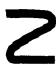
\includegraphics[keepaspectratio]{images/part001_ffa48347.jpg}}

Remarks. - 1) The relation (11) does not necessarily hold when \(\mathfrak{F}\) is an uncountable directed set of functions \(\geqslant 0\) that are not lower semi-continuous. Take for example \(X = R\) , \(\mu\) being Lebesgue measure on \(R\) , and consider the directed (for \(\leqslant\) ) set \(\mathfrak{F}\) of characteristic functions \(\varphi_{M}\) of all the finite subsets \(M\) of \(R\) . Then \(\mu^{*}(\varphi_{M}) = 0\) for every finite subset \(M\) , because a point is contained in an open interval of arbitrarily small length, and the characteristic function of a set reduced to a point therefore has upper integral zero by Def. 3 and Prop. 9 of No.~2. But the upper envelope of \(\mathfrak{F}\) is the constant function equal to 1, and \(\mu^{*}(1) = +\infty\) .

\begin{enumerate}
\def\labelenumi{\arabic{enumi})}
\setcounter{enumi}{1}
\tightlist
\item
  Note that for a decreasing sequence \((f_n)\) of functions \(\geqslant 0\) , one does not necessarily have \(\mu^{*}(\inf_{n} f_n) = \inf_{n} \mu^{*}(f_n)\) , even if \(\mu^{*}(f_n) < +\infty\) for all \(n\) (cf.~§4, Exer. 8 c)).
\end{enumerate}

PROPOSITION 13. --- For every sequence \((f_n)\) of numerical functions \(\geqslant 0\) defined on \(X\) ,

\[
\mu^ {*} \left(\sum_ {n = 1} ^ {\infty} f _ {n}\right) \leqslant \sum_ {n = 1} ^ {\infty} \mu^ {*} (f _ {n}).\tag{12}
\]

It suffices to apply the relation (10) to the increasing sequence of functions \(g_{n} = \sum_{k=1}^{n} f_{k}\) while taking into account that, by (9),

\[
\mu^ {*} (g _ {n}) \leqslant \sum_ {k = 1} ^ {n} \mu^ {*} (f _ {k}).
\]

In §5, No.~6, we will give conditions under which the two members of (12) are equal.

PROPOSITION 14 (Fatou's lemma). --- For every sequence \((f_{n})\) of numerical functions \(\geqslant 0\) ,

\[
\mu^ {*} \left(\liminf _ {n \to \infty} f _ {n}\right) \leqslant \liminf _ {n \to \infty} \mu^ {*} (f _ {n})  .\tag{13}
\]

For every integer \(n\) , set \(g_{n} = \inf_{p\geqslant 0}f_{n + p}\) ; the sequence \((g_n)\) is increasing and \(\liminf_{n\to \infty}f_n = \sup_n g_n\) , whence, by (10),

\[
\mu^ {*} (\liminf _ {n \to \infty} f _ {n}) = \sup _ {n} \mu^ {*} (g _ {n});
\]

but since \(g_{n} \leqslant f_{n+p}\) for \(p \geqslant 0\) , we have \(\mu^{*}(g_{n}) \leqslant \mu^{*}(f_{n+p})\) , whence \(\mu^{*}(g_{n}) \leqslant \inf_{p \geqslant 0} \mu^{*}(f_{n+p})\) and finally

\[
\mu^ {*} \left(\operatorname * {l i m i n f} _ {n \to \infty} f _ {n}\right) \leqslant \sup _ {n} \left(\inf _ {p \geqslant 0} \mu^ {*} (f _ {n + p})\right) = \operatorname * {l i m i n f} _ {n \to \infty} \mu^ {*} (f _ {n}).
\]

COROLLARY. --- Let \((f_{n})\) be a sequence of numerical functions \(\geqslant0\) such that, for every \(x\in X\) , \(\lim_{n\to\infty}f_{n}(x)=+\infty\) . If \(\mu\) is not the zero measure, then \(\lim_{n\to\infty}\mu^{*}(f_{n})=+\infty\) .

If \(f_{0}\) is the constant function equal to \(+\infty\) , then \(f_{0}\) is the upper envelope of all the functions of \(K_{+}\) , and, since \(\mu \neq 0\) , we have \(\mu^{*}(f_{0}) > 0\) ; but since \(f_{0} = \alpha f_{0}\) for every \(\alpha > 0\) , necessarily \(\mu^{*}(f_{0}) = +\infty\) (Prop. 11). The inequality (13) then shows that \(\mu^{*}(f_{n})\) tends to \(+\infty\) with n.

PROPOSITION 15. --- For every scalar \(\alpha > 0\) and every pair of positive measures \(\mu, \nu\) on \(X\) ,

\[
(\alpha \mu) ^ {*} = \alpha \mu^ {*}\tag{14}
\]

\[
(\mu + \nu) ^ {*} = \mu^ {*} + \nu^ {*}\tag{15}
\]

Moreover, the relation \(\mu \leqslant \nu\) implies \(\mu^{*} \leqslant \nu^{*}\) .

Let us prove the relation (15). Set \(\lambda = \mu + \nu\) ; thus \(\lambda(f) = \mu(f) + \nu(f)\) for \(f \in \mathcal{K}_+\) ; for \(f \in \mathcal{I}_+\) , the value of \(\lambda^*(f)\) (resp. \(\mu^*(f), \nu^*(f)\) ) is the limit of \(\lambda(g)\) (resp. \(\mu(g), \nu(g)\) ) as \(g\) runs over the directed set (for \(\leqslant\) ) of all \(g \in \mathcal{K}_+\) such that \(g \leqslant f\) ; therefore \(\lambda^*(f) = \mu^*(f) + \nu^*(f)\) . Finally, if \(f\) is any function \(\geqslant 0\) defined on X, then \(\lambda^*(f)\) (resp. \(\mu^*(f), \nu^*(f)\) ) is the limit of \(\lambda^*(h)\) (resp. \(\mu^*(h), \nu^*(h)\) ) as \(h\) runs over the directed set (for \(\geqslant\) ) of all functions \(h \in \mathcal{I}_+\) such that \(h \geqslant f\) ; again, by passage to the limit, we therefore have \(\lambda^*(f) = \mu^*(f) + \nu^*(f)\) , which proves (15). The relation (14) is established similarly. Finally, if \(\mu \leqslant \nu\) one can write \(\nu = \mu + (\nu - \mu)\) , where \(\nu - \mu \geqslant 0\) , therefore \(\nu^* = \mu^* + (\nu - \mu)^*\) , which shows that \(\mu^* \leqslant \nu^*\) .

\subsection{Outer measure of an arbitrary set}

DEFINITION 4. --- Let \(\mu\) be a positive measure on X; for every subset A of X, the upper integral \(\mu^{*}(\varphi_{\mathrm{A}})\) is called the outer measure of A (with respect to the measure \(\mu\) ) and is denoted \(\mu^{*}(\mathrm{A})\) .

The outer measure of a set is thus a number \(\geqslant0\) , finite or equal to \(+\infty\) , that, for an open set, coincides with the outer measure defined in Def. 2 of No.~2.

PROPOSITION 16. --- If A and B are two subsets of X such that A ⊂ B, then \(\mu^{*}(A) \leqslant \mu^{*}(B)\) .

COROLLARY. --- Every relatively compact set in X has finite outer measure.

For, such a set is contained in a relatively compact open set (GT, I, §9, No.~7, Prop. 10), whose outer measure is finite (No.~2, Prop. 5).

PROPOSITION 17. --- If \((\mathrm{A}_{n})\) is an increasing sequence of subsets of X, then \(\mu^{*}(\bigcup_{n}\mathrm{A}_{n})=\sup_{n}\mu^{*}(\mathrm{A}_{n})\) .

PROPOSITION 18. --- For every sequence (A \(_{n}\) ) of subsets of X,

\[
\mu^ {*} \left(\bigcup_ {n} \mathrm{A} _ {n}\right) \leqslant \sum_ {n} \mu^ {*} (\mathrm{A} _ {n}).
\]

These propositions are the translations of Props. 10 and 13 and of Th. 3 of No.~3 for characteristic functions of sets.

PROPOSITION 19. --- For every subset A of X, \(\mu^{*}(A)\) is the infimum of the outer measures of the open sets containing A.

The proposition is obvious if \(\mu^{*}(\mathbf{A}) = +\infty\) . In the contrary case, for every \(\varepsilon\) such that \(0 < \varepsilon < 1\) , there exists a function \(f \in \mathcal{I}_{+}\) such that \(\varphi_{\mathrm{A}} \leqslant f\) and \(\mu^{*}(\mathrm{A}) \leqslant \mu^{*}(f) \leqslant \mu^{*}(\mathrm{A}) + \varepsilon\) . Let \(\mathbf{G}\) be the set of \(x \in \mathbf{X}\) such that \(f(x) > 1 - \varepsilon\) . Since \(f\) is lower semi-continuous, \(\mathbf{G}\) is open (GT, IV, §6, No.~2, Prop. 1) and contains A; on the other hand \(f \geqslant (1 - \varepsilon)\varphi_{\mathrm{G}}\) , whence

\[
\mu^ {*} (\mathrm{G}) \leqslant \frac {1}{1 - \varepsilon} \mu^ {*} (f) \leqslant \frac {1}{1 - \varepsilon} \left(\mu^ {*} (\mathrm{A}) + \varepsilon\right);
\]

since \(\varepsilon\) is arbitrary, we see that \(\mu^{*}(\mathbf{G})\) differs as little as we please from \(\mu^{*}(\mathbf{A})\) , whence the proposition.

\section{NEGLIGIBLE FUNCTIONS AND SETS}

\subsection{Negligible positive functions}

DEFINITION 1. --- Given a measure \(\mu\) on a locally compact space \(X\) , a numerical function \(f \geqslant 0\) (finite or not) defined on \(X\) is said to be negligible for the measure \(\mu\) if \(|\mu|^*(f) = 0\) .

We then also say that f is \(\mu\) -negligible, or simply negligible if no confusion can result.

PROPOSITION 1. --- If \(f\) is a negligible function \(\geqslant 0\) , then every numerical function \(g\) such that \(0 \leqslant g \leqslant \alpha f\) ( \(\alpha\) a scalar \(> 0\) ) is negligible.

For, \(0 \leqslant |\mu|^*(g) \leqslant \alpha |\mu|^*(f) = 0\)

PROPOSITION 2. --- The sum and upper envelope of a sequence \((f_{n})\) of negligible functions \(\geqslant0\) are negligible.

For, \(|\mu|^*(\sum_n f_n) \leqslant \sum_n |\mu|^*(f_n) = 0\) (§1, No.~3, Prop. 13) and \(\sup_n f_n \leqslant \sum_n f_n\) .

PROPOSITION 3. --- For a lower semi-continuous function \(f \geqslant 0\) on \(X\) to be negligible, it is necessary and sufficient that \(f\) be zero on the support of \(\mu\) .

If \(|\mu|^*(f) = 0\) then \(|\mu|(g) = 0\) for every function \(g \in \mathcal{H}_+\) such that \(g \leqslant f\) ; it follows (Ch. III, §2, No.~3, Prop. 9) that \(g\) is zero on the support S of \(\mu\) ; since \(f\) is the upper envelope of the functions \(g \in \mathcal{H}_+\) such that \(g \leqslant f\) (§1, No.~1, Lemma), \(f(x) = 0\) on S. Conversely, if \(f(x) = 0\) on S then \(g(x) = 0\) on S for every function \(g \in \mathcal{H}_+\) such that \(g \leqslant f\) , therefore (Ch. III, §2, No.~3, Prop. 8) \(|\mu|(g) = 0\) , which, by definition, implies that \(|\mu|^*(f) = 0\) .

\subsection{Negligible sets}

DEFINITION 2. --- Given a measure \(\mu\) on a locally compact space \(X\) , a subset \(A\) of \(X\) is said to be negligible for the measure \(\mu\) if \(|\mu|^*(A) = 0\) .

One also says that A is \(\mu\) -negligible, or simply negligible if no confusion can result. It comes to the same thing to say that the characteristic function \(\varphi_{A}\) is negligible.

PROPOSITION 4. --- Every subset of a negligible set is negligible; every countable union of negligible sets is negligible.

This is an immediate consequence of Props. 1 and 2.

Example. --- Let \(\mu\) be Lebesgue measure on R. Every set \(\{x_{0}\}\) reduced to a point is negligible (cf.~§1, No.~3, Remark 1). It follows that every countable subset of R is negligible for Lebesgue measure. The converse of this proposition is incorrect (§4, Exer. 4 b)).

PROPOSITION 5. --- The complement of the support S of \(\mu\) is the largest negligible open set in X.

For, by Prop. 3, in order that an open set G be negligible, it is necessary and sufficient that \(G \cap S = \varnothing\) , that is, \(G \subset CS\) .

\subsection{Properties true almost everywhere}

Let X be a locally compact space, \(\mu\) a measure on X. If \(P\{x\}\) is a property, the property \(\langle P\{x\}\) almost everywhere (with respect to \(\mu\) ) is by definition equivalent to the property \(\langle\) the set of x such that \((x \in X \text{ and not } P\{x\})\) is \(\mu\) -negligible.

THEOREM 1. --- In order that a numerical function (finite or not) \(f \geqslant 0\) defined on X be negligible, it is necessary and sufficient that \(f(x) = 0\) almost everywhere.

The condition is necessary. For, suppose that \(f\) is negligible, and let \(N\) be the set of \(x \in X\) such that \(f(x) \neq 0\) ; then \(\varphi_N \leqslant \sup_n (nf)\) , therefore \(\varphi_N\) is negligible (No.~1, Props. 1 and 2).

The condition is sufficient. Suppose that the set N of points where \(f(x) \neq 0\) is negligible; then \(f \leqslant \sup_{n} n\varphi_{N}\) , therefore f is negligible (No.~1, Props. 1 and 2).

PROPOSITION 6. --- If \(f\) and \(g\) are two functions \(\geqslant 0\) (finite or not) defined on X such that \(f(x) = g(x)\) almost everywhere, then \(|\mu|^*(f) = |\mu|^*(g)\) .

Let N be the negligible set of points \(x \in X\) such that \(f(x) \neq g(x)\) . The functions \(\inf(f, g)\) and \(\sup(f, g)\) being equal except at the points of N, it suffices to prove the proposition assuming \(f \leqslant g\) . Let h be the function equal to \(+\infty\) at the points of N, and to 0 on CN; then \(f \leqslant g \leqslant f + h\) , thus

\[
| \mu | ^ {*} (f) \leqslant | \mu | ^ {*} (g) \leqslant | \mu | ^ {*} (f + h) \leqslant | \mu | ^ {*} (f) + | \mu | ^ {*} (h) = | \mu | ^ {*} (f)
\]

(since \(h\) is negligible), whence the proposition.

PROPOSITION 7. --- If \(f\) is a function \(\geqslant 0\) defined on \(X\) such that \(|\mu|^*(f) < +\infty\) , then \(f(x)\) is finite almost everywhere.

For, let N be the set of points \(x \in X\) such that \(f(x) = +\infty\) ; for every integer n, \(n\varphi_{N} \leqslant f\) , whence \(n|\mu|^{*}(\varphi_{N}) \leqslant |\mu|^{*}(f)\) ; since n is arbitrarily large, \(|\mu|^{*}(N) = 0\) .

However, even if X is compact, a function \(f \geqslant 0\) defined on X and everywhere finite can have infinite upper integral, as is shown by the example X = {[}0, 1{]}, \(f(x) = 1/x\) for x \textgreater{} 0 and \(f(0) = 0\) , \(\mu\) being Lebesgue measure on X.

\subsection{Classes of equivalent functions}

Let \(\mu\) be a measure on a locally compact space \(X\) . Given a set \(F\) , two mappings \(f, g\) of \(X\) into \(F\) are said to be equivalent with respect to \(\mu\) (or \(\mu\) -equivalent, or simply equivalent if no confusion can arise) if \(f(x) = g(x)\) almost everywhere in \(X\) . Since the union of two negligible sets is negligible, one indeed defines in this way an equivalence relation in the set \(F^X\) of all mappings of \(X\) into \(F\) ; when we speak of the equivalence class of such a function \(f\) (without further specification) it will be understood to be the class of all the functions equal almost everywhere to \(f\) ; in this chapter and those that follow, we will indicate this class by the notation \(\widetilde{f}\) .

PROPOSITION 8. --- Let \((\mathrm{F}_{n})\) be a countable family (finite or infinite) of sets. For every index n, let \(f_{n}, g_{n}\) be two equivalent mappings of X into \(F_{n}\) ; then, there exists a negligible set H such that, for every \(x \notin H\) , \(f_{n}(x) = g_{n}(x)\) for all n.

For, the set \(H_{n}\) of \(x \in X\) such that \(f_{n}(x) \neq g_{n}(x)\) is negligible, therefore so is their union H (No.~2, Prop. 4), and this set meets the requirements.

COROLLARY. --- If \(\varphi\) is a mapping of \(\prod_{n} F_n\) into a set \(G\) , then the mappings \(\varphi((f_n))\) and \(\varphi((g_n))\) of \(X\) into \(G\) are equivalent.

We denote by \(\varphi((\widetilde{f}_n))\) the equivalence class of every function \(\varphi((f_n))\) , where \(f_n\) is an arbitrary function in the class \(\widetilde{f}_n\) .

In particular, if F is a vector space over R, one defines \(\widetilde{f} + \widetilde{g}\) and \(\alpha\widetilde{f}\) to be the equivalence classes of \(f + g\) and \(\alpha f\) , respectively (f and g being mappings of X into F, and \(\alpha\) a scalar); we obtain in this way, on the set of equivalence classes of mappings of X into F, a vector space structure: moreover, this is the quotient space structure of that of \(F^{X}\) by the linear subspace of mappings f such that \(\widetilde{f} = \widetilde{0}\) (the functions that are zero almost everywhere), which we also call negligible functions (with values in F). One defines similarly the product \(\widetilde{g}\widetilde{f}\) , where \(\widetilde{f}\) is an equivalence class of mappings of X into F, and \(\widetilde{g}\) is an equivalence class of (finite) numerical functions defined on X: the set of equivalence classes of mappings of X into F is thus equipped with the structure of a module over the set of equivalence classes of finite numerical functions defined on X (which is itself equipped with a ring structure). If F is an algebra over R, one defines similarly an algebra structure on the set of equivalence classes of mappings of X into F.

Let F be a metrizable topological space, and consider a uniform structure on F compatible with its topology and defined by a countable family of pseudometrics \(\rho_{n}\) (GT, IX, §§1 and 2); in order that two mappings f, g of X into F be equivalent, it is necessary and sufficient that the numerical functions \(\rho_{n}(f,g)\) be negligible; for, this is equivalent to saying that there exists a negligible set H in X such that, for every \(x\notin H\) , \(\rho_{n}(f(x),g(x))=0\) for all n, that is, \(f(x)=g(x)\) . In particular, if F is a metrizable locally convex space, and \((q_{n})\) is a countable family of seminorms defining the topology of F (TVS, II, §4, No.~1), in order that two mappings f, g of X into F be equivalent it is necessary and sufficient that all of the numerical functions \(q_{n}(\mathbf{f}(x)-\mathbf{g}(x))\) be negligible.

PROPOSITION 9. --- Let f and g be two continuous mappings of X into a Hausdorff topological space F; for f and g to be equivalent, it is necessary and sufficient that \(f(x) = g(x)\) at every point of the support of \(\mu\) .

For, the set of \(x \in X\) such that \(f(x) \neq g(x)\) is an open set (GT, I, §8, No.~1); for it to be negligible, it is necessary and sufficient that it not intersect the support of \(\mu\) (No.~2, Prop. 5).

PROPOSITION 10. --- Let F be a Hausdorff locally convex space over R such that there exists in the dual F' of F a sequence ( \(a_{n}^{\prime}\) ) that is dense for the weak topology \(\sigma(F^{\prime},F)\) (TVS, II, §6, No.~2). In order that two mappings f, g of X into F be equivalent, it is necessary and sufficient that, for every n, the numerical functions \(\langle\mathbf{f}(x),\mathbf{a}_{n}^{\prime}\rangle\) and \(\langle\mathbf{g}(x),\mathbf{a}_{n}^{\prime}\rangle\) be equivalent.

The condition is obviously necessary. Conversely, if it is satisfied, there exists a negligible set H such that, for each \(x \notin H\) , \(\langle \mathbf{f}(x), \mathbf{a}_{n}^{\prime} \rangle = \langle \mathbf{g}(x), \mathbf{a}_{n}^{\prime} \rangle\) for every n; this means that the weakly continuous linear forms \(\mathbf{z}^{\prime} \mapsto \langle \mathbf{f}(x), \mathbf{z}^{\prime} \rangle\) and \(\mathbf{z}^{\prime} \mapsto \langle \mathbf{g}(x), \mathbf{z}^{\prime} \rangle\) on \(F^{\prime}\) are equal at each of the points \(a_{n}^{\prime}\) , hence are identical by virtue of the hypothesis, which proves that \(\mathbf{f}(x) = \mathbf{g}(x)\) for all \(x \notin H\) .

Note that the hypothesis of Prop. 10 is applicable in particular when F is a locally convex space that is metrizable and separable \(^{1}\) (TVS, III, §3, No.~4, Cor. 2 of Prop. 6).

\subsection{Functions defined almost everywhere}

In conformity with the definition in No.~3, a mapping f of a subset A of X into a set F is said to be defined almost everywhere if the complement of the set A on which it is defined is a negligible set. We again call equivalence class of f, and denote by \(\widetilde{f}\) , the equivalence class of every function defined on all of X and equal to \(f(x)\) at the points \(x \in X\) where f is defined; it is clear that this class depends only on f.~Two functions f, g defined almost everywhere are again said to be equivalent if \(\widetilde{f} = \widetilde{g}\) : this means, therefore, that the set of points where \(f(x)\) and \(g(x)\) are both defined and equal has negligible complement.

It follows at once that Prop. 8 of No.~4 and its corollary may be generalized to the case where in their statements it is assumed only that each of the functions \(f_{n}, g_{n}\) is defined almost everywhere; then the functions \(\varphi((f_{n}))\)

and \(\varphi((g_n))\) are themselves defined almost everywhere; the equivalence class of \(\varphi((f_n))\) is again \(\varphi((\widetilde{f}_n))\) .

A function defined almost everywhere, with values in a vector space F, is again said to be negligible if it is equivalent to 0. If f is a negligible function with values in F, and u is a linear mapping of F into a vector space G, then the composite function \(u \circ f\) (defined almost everywhere) is negligible; similarly, for every (finite) numerical function g, defined almost everywhere, the function gf (defined almost everywhere) is negligible.

\pandocbounded{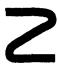
\includegraphics[keepaspectratio]{images/part001_e94daaaa.jpg}}

One must take care to observe that, in the set of functions with values in F and defined almost everywhere, the internal law of composition \((\mathbf{f},\mathbf{g})\mapsto\mathbf{f}+\mathbf{g}\) is not a group law, because, while the function 0 is indeed a neutral element for this law, if f is not everywhere defined then there does not exist a function g such that \(f+g=0\) . This is what motivates the introduction of the equivalence classes \(\widetilde{f}\) , which do form a vector space.

Let \((f_n)\) be a sequence of mappings into a topological space F, each of which is defined almost everywhere in X. We say that the sequence \((f_n)\) converges (pointwise) almost everywhere to f in X if the set of points \(x \in X\) where all the \(f_n(x)\) are defined and the sequence \((f_n(x))\) has a limit equal to \(f(x)\) , has negligible complement. It is clear that if, for each n, the function \(g_n\) (defined almost everywhere) is equivalent to \(f_n\) , then the sequence \((g_n)\) converges almost everywhere to f.

If F is topological vector space, one defines similarly an almost everywhere convergent series, whose general term is a function \(f_{n}\) defined almost everywhere in X with values in F; the sum of this series is a function defined at the points where the partial sums \(\sum_{k=1}^{n}\mathbf{f}_{k}(x)\) are defined and have a limit, and its class depends only on the classes \(\widetilde{f}_{n}\) .

\subsection{\texorpdfstring{Equivalence classes of functions with values in \(\overline{R}\)}{Equivalence classes of functions with values in R-bar}}

In conformity with the definition in No.~3, we say that a function \(f\) , defined almost everywhere in \(X\) and with values in \(\overline{\mathbf{R}}\) , is finite almost everywhere if the set of \(x \in X\) for which \(f(x)\) is defined and finite has negligible complement. A function that is finite almost everywhere is equivalent to a function that is everywhere finite; one can therefore identify its class \(\widetilde{f}\) with a class of finite numerical functions defined on \(X\) (or almost everywhere in \(X\) ). In particular, the sum and product of two classes of functions finite almost everywhere are defined, and the set of these classes is an algebra over \(\mathbf{R}\) . If \((f_n)\) is a sequence of functions with values in \(\overline{\mathbf{R}}\) , defined and finite almost everywhere, then the partial sums \(\sum_{k=1}^{n} f_k(x)\) are defined almost everywhere; if, for almost every \(x \in X\) , they have a limit \(f(x)\) in \(\overline{R}\) , we again say that the series with general term \(f_{n}\) converges almost everywhere and that f is the sum of the series (note that f is not necessarily finite almost everywhere).

If \(f\) and \(g\) are two numerical functions defined and finite almost everywhere in \(X\) , then \(\widetilde{f} + \widetilde{g}\) (resp. \(\widetilde{f}\widetilde{g}\) ) is the class of every function equal to \(f(x) + g(x)\) (resp. \(f(x)g(x)\) ) at the points \(x \in X\) where this expression has meaning. Note that \(f\) and \(g\) can both be everywhere defined without \(f(x) + g(x)\) (resp. \(f(x)g(x)\) ) being defined for all \(x\) (GT, IV, §4, No.~3); by definition \(f + g\) (resp. \(fg\) ) is then the function equal to \(f(x) + g(x)\) (resp. \(f(x)g(x)\) ) at the points where this expression is defined; it is therefore only defined almost everywhere.

Let \(f\) and \(g\) be two numerical functions (finite or not) defined almost everywhere in \(X\) and such that \(f(x) \leqslant g(x)\) almost everywhere; if \(f_1\) is equivalent to \(f\) , and \(g_1\) is equivalent to \(g\) , it is clear that also \(f_1(x) \leqslant g_1(x)\) almost everywhere. The relation in question therefore depends only on the classes of \(f\) and \(g\) ; one writes \(\widetilde{f} \leqslant \widetilde{g}\) , and one verifies immediately that this relation is an order relation in the set of equivalence classes of functions with values in \(\overline{\mathbf{R}}\) . If \((\widetilde{f}_n)\) is a countable family (finite or infinite) of such classes and if, for every \(n\) , \(f_n\) and \(g_n\) are two functions defined almost everywhere and belonging to the class \(\widetilde{f}_n\) , it follows from Prop. 8 of No.~4 that the functions \(\sup_n f_n\) and \(\sup_n g_n\) , defined almost everywhere, are equivalent; their class therefore depends only on the classes \(\widetilde{f}_n\) , and one verifies at once that it is the supremum \(\sup_n \widetilde{f}_n\) of these classes in the set of classes of functions with values in \(\overline{\mathbf{R}}\) , ordered in the way just described (a set which is therefore, in particular, lattice-ordered). One shows similarly the existence of the infimum \(\inf_n \widetilde{f}_n\) , and one has \(\inf_n \widetilde{f}_n = -\sup_n (-\widetilde{f}_n)\) . It follows that \(\limsup_{n \to \infty} f_n\) and \(\limsup_{n \to \infty} g_n\) are also equivalent, and their class, which is denoted \(\limsup_{n \to \infty} \widetilde{f}_n\) , is equal to \(\inf_n (\sup_{p \geqslant 0} \widetilde{f}_{n+p})\) ; \(\liminf_{n \to \infty} \widetilde{f}_n\) is defined similarly.

A numerical function f (finite or not) is said to be negligible if it is equivalent to 0; this definition is equivalent to Def. 1 for functions that are positive and everywhere defined, by virtue of Th. 1. For f to be negligible, it is necessary and sufficient that \(|f|\) be negligible (or that both \(f^{+}\) and \(f^{-}\) be negligible).

\section{\texorpdfstring{\(\mathrm{L}^{p}\) SPACES}{L to the p spaces}}
